\documentclass[a4paper]{article}
\usepackage[utf8]{inputenc}
\usepackage[spanish, es-tabla, es-noshorthands]{babel}
\usepackage[table,xcdraw]{xcolor}
\usepackage[a4paper, footnotesep = 1cm, width=20cm, top=2.5cm, height=25cm, textwidth=18cm, textheight=25cm]{geometry}
%\geometry{showframe}

\usepackage{tikz}
\usepackage{amsmath}
\usepackage{amsfonts}
\usepackage{amssymb}
\usepackage{float}
\usepackage{graphicx}
\usepackage{caption}
\usepackage{subcaption}
\usepackage{multicol}
\usepackage{multirow}
\setlength{\doublerulesep}{\arrayrulewidth}
\usepackage{booktabs}

\usepackage{hyperref}
\hypersetup{
    colorlinks=true,
    linkcolor=blue,
    filecolor=magenta,      
    urlcolor=blue,
    citecolor=blue,    
}

\newcommand{\quotes}[1]{``#1''}
\usepackage{array}
\newcolumntype{C}[1]{>{\centering\let\newline\\\arraybackslash\hspace{0pt}}m{#1}}
\usepackage[american]{circuitikz}
\usetikzlibrary{calc}
\usepackage{fancyhdr}
\usepackage{units} 

\graphicspath{{../Ejercicio-1/}{../Ejercicio-2/}{../Ejercicio-3/}{../Ejercicio-4/}}

\pagestyle{fancy}
\fancyhf{}
\lhead{22.01 Teoría de Circuitos}
\rhead{Mechoulam, Lambertucci, Rodriguez Turco, Londero, Galdeman}
\rfoot{\centering \thepage}

\begin{document}

%%%%%%%%%%%%%%%%%%%%%%%%%%%%%%%%%%%%%%%%%%%%%%%%%%%%%%%%%%%%%%%%%%%%%%%%% 
%								CARATULA								%
%%%%%%%%%%%%%%%%%%%%%%%%%%%%%%%%%%%%%%%%%%%%%%%%%%%%%%%%%%%%%%%%%%%%%%%%% 

\begin{titlepage}
\newcommand{\HRule}{\rule{\linewidth}{0.5mm}}
\center
\mbox{\textsc{\LARGE \bfseries {Instituto Tecnológico de Buenos Aires}}}\\[1.5cm]
\textsc{\Large 22.01 Teoría de Circuitos}\\[0.5cm]


\HRule \\[0.6cm]
{ \Huge \bfseries Trabajo práctico N$^{\circ}$5}\\[0.4cm] 
\HRule \\[1.5cm]


{\large

\emph{Grupo 3}\\
\vspace{3px}

\begin{tabular}{lr} 	
\textsc{Mechoulam}, Alan  &  58438\\
\textsc{Lambertucci}, Guido Enrique  & 58009 \\
\textsc{Rodriguez Turco}, Martín Sebastian  & 56629 \\
\textsc{Londero Bonaparte}, Tomás Guillermo  & 58150 \\
\textsc{Galdeman}, Agustín & 59827\\
\end{tabular}

\vspace{20px}

\emph{Profesores}\\
Jacoby, Daniel Andrés\\
Belaustegui Goitia, Carlos\\
Iribarren, Rodrigo Iñaki\\
\vspace{3px}
%\textsc{} \\	

\vspace{100px}

\begin{tabular}{ll}

Presentado: & */*/19\\

\end{tabular}

}

\vfill

\end{titlepage}


%%%%%%%%%%%%%%%%%%%%%%%%%%%%%%%%%%%%%%%%%%%%%%%%%%%%%%%%%%%%%%%%%%%%%%%%% 
%								INFORME									%
%%%%%%%%%%%%%%%%%%%%%%%%%%%%%%%%%%%%%%%%%%%%%%%%%%%%%%%%%%%%%%%%%%%%%%%%%

\section{Introducción}

\section{Desarrollo}

\subsection{Comportamiento de Amplificadores Operacionales}

	\documentclass[a4paper]{article}
\usepackage[utf8]{inputenc}
\usepackage[spanish, es-tabla, es-noshorthands]{babel}
\usepackage[table,xcdraw]{xcolor}
\usepackage[a4paper, footnotesep = 1cm, width=20cm, top=2.5cm, height=25cm, textwidth=18cm, textheight=25cm]{geometry}
%\geometry{showframe}

\usepackage{tikz}
\usepackage{amsmath}
\usepackage{amsfonts}
\usepackage{amssymb}
\usepackage{float}
\usepackage{graphicx}
\usepackage{caption}
\usepackage{subcaption}
\usepackage{multicol}
\usepackage{multirow}
\setlength{\doublerulesep}{\arrayrulewidth}
\usepackage{booktabs}

\usepackage{hyperref}
\hypersetup{
    colorlinks=true,
    linkcolor=blue,
    filecolor=magenta,      
    urlcolor=blue,
    citecolor=blue,    
}

\newcommand{\quotes}[1]{``#1''}
\usepackage{array}
\newcolumntype{C}[1]{>{\centering\let\newline\\\arraybackslash\hspace{0pt}}m{#1}}
\usepackage[american]{circuitikz}
\usetikzlibrary{calc}
\usepackage{fancyhdr}
\usepackage{units} 

\graphicspath{{../Ejercicio-1/}{../Ejercicio-2/}{../Ejercicio-3/}{../Ejercicio-4/}}

\pagestyle{fancy}
\fancyhf{}
\lhead{22.01 Teoría de Circuitos}
\rhead{Mechoulam, Lambertucci, Rodriguez Turco, Londero, Galdeman}
\rfoot{\centering \thepage}

\newcommand\underrel[2]{\mathrel{\mathop{#2}\limits_{#1}}}

\usepackage{circuitikz}
\usepackage{xcolor}
\usepackage{amsmath}

\begin{document}


\section{Comportamiento de Amplificadores Operacionales.}

\subsection{Introducción y modelos.}
En el presente punto se analizan las limitaciones del amplificador operacional \textbf{LM324} en las configuraciones inversora y no inversora.

Un amplificador operacional es un dispositivo electrónico el cual, dependiendo de la tensión de entrada, fija una tensión de salida. Estos se pueden modelar de la siguiente forma:
\begin{figure}[H]	
	\centering
	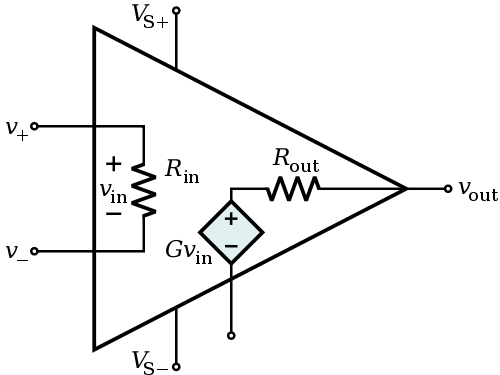
\includegraphics[width=0.7\textwidth]{Ejercicio1/Imagenes/Basicopamp.png}
	\caption{Modelo básico del amplificador operacional.}
	\label{fig:Basicopamp}
\end{figure}
donde típicamente $R_{in}\approx \infty$ y $R_{out} \approx 0$

\subsubsection{Modelo ideal.}
En el modelo ideal realimentado por el borne inversor ($V^-$), las hipótesis con las que se trabaja son:
\begin{align} V^+ = V^- \end{align}
\begin{align}V_{Out} \underrel{A_{Vol}\to \infty}{=} A_{Vol} \cdot (V^+ - V^-) \end{align}
\begin{align} R_{in}=\infty   \thinspace;\thinspace R_{Out} = 0 \end{align}


\subsubsection{Modelo $A_{Vol}$ finito.}
Para este modelo se le agregan idealidades al modelo anterior.
\begin{align}V_{Out} = A_{Vol} \cdot (V^+ - V^-)
\label{eq:vout}
\end{align}

Si bien la realimentación negativa intentará hacer que la diferencia entre $V^+$ y $V^-$ sea 0, no es algo que se asume en este modelo.

\subsubsection{Modelo polo dominante.}
Este modelo es el más cercano al real que se trata en el presente trabajo. Los amplificadores operacionales poseen un polo dominante, el cual está diseñado intencionalmente por el fabricante, para cubrir algunos problemas que surgen al trabajar con mayores frecuencias. Estos dispositivos cuentan con una serie de polos debido a capacidades parásitas propias de la construcción. El polo dominante es introducido para evitar que estos polos desestabilicen el circuito al introducir una inversión en el lazo de realimentación, a altas frecuencias.

\begin{figure}[H]	
	\centering
	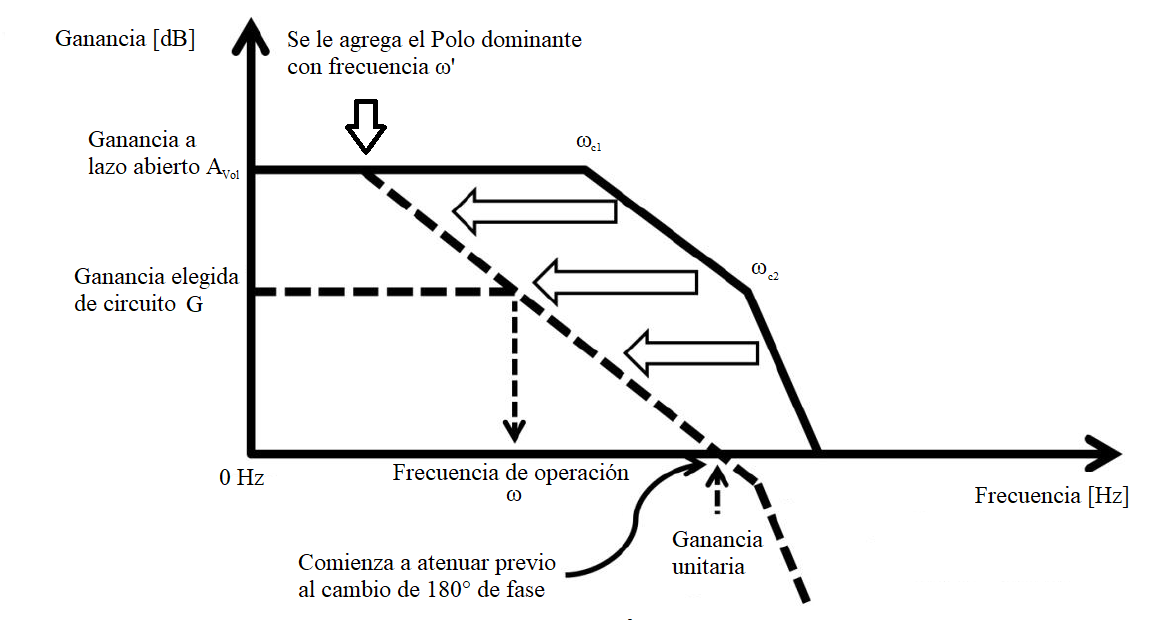
\includegraphics[width=\textwidth]{Ejercicio1/Imagenes/dompole.png}
	\caption{Modelo polo dominante.}
	\label{fig:dompole}
\end{figure}

También se define un ``Ancho de Banda'', con el cual se puede trabajar; comúnmente el dato con el que se trabaja es el conocido como GBP (Gain Bandwidth Product), el cual sigue la siguiente relación:

\begin{align} GBP= A_{Vol} \cdot \omega' \end{align}
donde $\omega'$ es la frecuencia del polo dominante a lazo abierto. También se cumple que 

\begin{align} GBP=\omega \cdot G \end{align}
donde $\omega$ es la frecuencia de corte del circuito en el que esté aplicado y G la ganancia del mismo.
Finalmente la ecuación principal que rige este modelo es (\ref{eq:vout}) con la singularidad de que:
\begin{equation}
	A_{Vol} = A_{Vol}(s) = \frac{A_{vol}}{1+\frac{s}{\omega '}}
	\label{eq:PoloDom}
\end{equation}  

\subsection{Configuración inversora y no inversora.}
La cátedra propone dos modelos de circuitos diferentes para analizar. Estos son los presentados a continuación:

\begin{figure}[H]
\begin{center}
\begin{circuitikz}
	\node [op amp](A1){};
	\draw (A1.-) to[short] ++(-2.5,0) to[R, l_= $R_1$] ++(-1.5,0) to[short, -o] node[ocirc,label=left:$V_{in}$]{} ++(-1,0);
	\draw (A1.-) to[open] ++(-2,0) to[R, l_= $R_3$] ++(0,-2) node[ground]{};
	\draw (A1.-) node[label=south:$V^-$]{};
	\draw (A1.+) node[label=south:$V^+$]{};
	\draw (A1.+) to[short] ++(-1,0) to[short] ++(0,-1) node[ground]{};
	\draw (A1.-) to[short] ++(0,1.5) to[R, l = $R_2$] ++(3,0) to[short] ++(0,-2) to[R, l = $R_4$] ++(0,-1.5) node[ground]{};
	\draw (A1.out) to[short, -o] ++(1,0) node[ocirc,label=right:$V_{out}$]{};
	\end{circuitikz}
	\caption{Configuración inversora.}
	\label{fig:ConfInv}
\end{center}
\end{figure}

\begin{figure}[H]
\begin{center}
\begin{circuitikz}
	\node [op amp](A1){};
	\draw (A1.-) to[short] ++(-1.5,0) to[R, l_=$R_1$] ++(-1.5,0) to[short] ++(-1,0) node[ground]{};
	\draw (A1.-) node[label=south:$V^-$]{};
	\draw (A1.+) node[label=south:$V^+$]{};
	\draw (A1.-) to[short] ++(0,1.5) to[R, l = $R_2$] ++(3,0) to[short] ++(0,-2);
	\draw (A1.+) to[short] ++(-1,0) to[R, l = $R_4$] ++(0,-1.5) node[ground]{};
	\draw (A1.out) to[short, -o] ++(1,0) node[ocirc,label=right:$V_{out}$]{};
	\draw (A1.+) to[short] ++(-1,0) to[R, l= $R_3$] ++(-2,0) to[short, -o] node[ocirc,label=left:$V_{in}$]{} ++(-1,0);
	\end{circuitikz}
	\caption{Configuración no inversora.}
	\label{fig:ConfNoInv}
\end{center}
\end{figure}

Para ambos, y debido a que se utiliza el mismo operacional en cada caso, se obtuvieron los siguientes datos de la hoja de datos del fabricante:
\begin{table}[H]
\begin{center}
\begin{tabular}{|c|c|c|c|c|}
\hline
%\multicolumn{5}{|c|}{}                                      \\ \hline
\textbf{$A_{vol}$} & $Max \ V_{in}$ & $V_{cm}$ & Slew rate             & GBW \\ \hline
100 k              & $32 \ V$         & $VCC \ - \ 1.5 \ V$  & 0.3 $\frac{V}{\mu s}$ & $1 \ MHz$  \\ \hline
\end{tabular}
\caption{Datos pertinentes al operacional.}
\label{tab:datos}
\end{center}
\end{table}

%%%%%%%%%%%%%%%%%%%%%%%%%%%%
\subsubsection{Calculo Analítico del Circuito Inversor.}
Lo primero que se realizó fue utilizar el equivalente de Thevenin para simplificar los cálculos analíticos.

\begin{figure}[H]
\begin{center}
\begin{circuitikz}
	\node [op amp](A1){};
	\draw (A1.-) to[short] ++(-1,0) to[R, l = $R_{Thevenin}$] ++(-2,0) to[short, -o] node[ocirc,label=left:$V_{Thevenin}$]{} ++(-0.5,0);
	\draw (A1.-) node[label=south:$V^-$]{};
	\draw (A1.+) node[label=south:$V^+$]{};
	\draw (A1.+) to[short] ++(-1,0) to[short] ++(0,-1) node[ground]{};
	\draw (A1.-) to[short] ++(0,1.5) to[R, l = $R_2$] ++(3,0) to[short] ++(0,-2) to[R, l = $R_4$] ++(0,-1.5) node[ground]{};
	\draw (A1.out) to[short, -o] ++(2,0) node[ocirc,label=right:$V_{out}$]{};
	\end{circuitikz}
	\caption{Equivalente de Thevenin del circuito inversor.}
	\label{fig:Thevenin}
\end{center}
\end{figure}

Teniendo en cuenta que 
\begin{align}
	V_{Thevenin} = V_{in} \cdot \frac{R_3}{R_1+R_3} \\
	R_{Thevenin} = \frac{R_1\cdot R_3}{R_1+R_3}
\label{eq:thev}
\end{align} 

Se considera primero caso genérico y una vez terminado el desarrollo, se toman las aproximaciones necesarias para los diversos casos pedidos.
\begin{align}
V_{Out}= A_{Vol}(\omega) \cdot (V^+ - V^-)
\label{equ:avoligualvo}
\end{align}
\begin{align}
V^+=0\end{align}
\begin{align}\frac{V_{Th}-V^-}{R_{Th}}=\frac{V^--V_{Out}}{R_2}
\label{eq:nodeInv}
\end{align}

Despejando para $V_{Out}$ se llega a que:
\begin{align}
\label{eq:Vout}
V_{Out}=-V_{in} \cdot \frac{R_3}{R_1+R_3} \cdot \frac{\frac{R_2}{R_{Th}+R_2}\cdot A(\omega)}{1+\frac{R_{Th}}{R_{Th}+R_2}\cdot A(\omega)}
\end{align}
sabiendo que la transferencia es $ H(s)=\frac{V_{Out}}{V_{in}} $.

Para el caso de $A_{Vol}=\infty$ simplemente basta tomar:
\begin{align}\lim_{A_{Vol}\to\infty} - \frac{R_3}{R_1+R_3} \cdot \frac{\frac{R_2}{R_{Th}+R_2}\cdot A(\omega)}{1+\frac{R_{Th}}{R_{Th}+R_2}\cdot A(\omega)} = -\frac{R_3}{R_1+R_3}\cdot\frac{R_2}{R_{Th}}=-\frac{R_2}{R_1}\end{align}

Para el caso de $A_{Vol}$ finito solamente se reescribirá (\ref{eq:Vout}).

\begin{align}
H(s)= -\frac{R_2\cdot A_{Vol}}{R_1\cdot R_3+R_1\cdot R_3 \cdot A_{Vol} +R_2\cdot R_3+R_2\cdot R_1}
\label{eq:AvolFinite}
\end{align}

Finalmente el caso el cual incluye el polo dominante alcanza con tomar lo especificado en (\ref{eq:PoloDom}), donde $\omega'$ es la frecuencia del polo dominante. Utilizando (\ref{eq:PoloDom}) y (\ref{eq:AvolFinite}) se llega a la expresión:
\begin{align}
\label{eq:polodom}
H(s)=-\frac{A_0R_2R_3}{A_0R_1R_3+R_1R_2+R_1R_3+R_2R_3} \cdot \left[1+s \left( \omega' \cdot \frac{A_0R_1R_3+R_1R_2+R_1R_3+R_2R_3}{R_1R_2+R_1R_3+R_2R_3} \right)^{-1} \right]^{-1}
\end{align}

De (\ref{eq:polodom}) se obtiene la frecuencia de corte del sistema.
\begin{align}
f_c=\frac{\omega'}{2\pi} \cdot \frac{A_0R_1R_3+R_1R_2+R_1R_3+R_2R_3}{R_1R_2+R_1R_3+R_2R_3}
\end{align}
Luego, teniendo en cuenta que
\begin{align}
\omega'=\frac{GBW}{A_0} = 2 \pi\cdot 10 \ Hz \approx 62.83 \ Hz
\end{align}

Para este grupo, los valores de resistencias asignados se presentan a continuación:
\begin{table}[H]
\begin{center}
\begin{tabular}{|c|c|c|c|}
\hline
\textbf{Caso:}              & \textbf{1}               & \textbf{2}               & \textbf{3}                \\ \hline
$R_1=R_3$                   & $7.5$                      & $7.5$                      & $75$                       \\ \hline
$R_2$                       & $75$                       & $7.5$                      & $7.5$                       \\ \hline
\multicolumn{1}{|c|}{$R_4$} & \multicolumn{1}{l|}{$30$} & \multicolumn{1}{l|}{$30$} & \multicolumn{1}{l|}{$300$} \\ \hline
\end{tabular}
\caption{Valores de resistencias en $k\Omega$.}
\label{tabla:resasignadas}
\end{center}
\end{table}

Para estos casos se calculó la ganancia considerando $A_{Vol}$ finito e infinito. Además, se calculó la frecuencia de corte del sistema para $A(\omega)$.

\begin{table}[H]
\begin{center}
\begin{tabular}{|c|c|c|c|}
\hline
\textbf{Caso}            & \textbf{1} & \textbf{2} & \textbf{3} \\ \hline
\textbf{$H(s)_{\infty}$} & 10         & 1          & 0.1        \\ \hline
\textbf{$H(s)_{Finito}$} & 9.9998     & 0.9999     & 0.0999     \\ \hline
\textbf{$f_c$}           & 47.62 kHz   & 333.34 kHz  & 833.34 kHz     \\ \hline
\end{tabular}
\caption{Ganancias y frecuencias de corte de los circuitos inversores.}
\label{tabla:gananciasinv}
\end{center}
\end{table}

Luego se procedió a realizar los gráficos de $H(s)$ cpn las distintas consideraciones de $A_{Vol}$ para cada uno de los 3 casos.
\begin{figure}[H]	
	\centering
	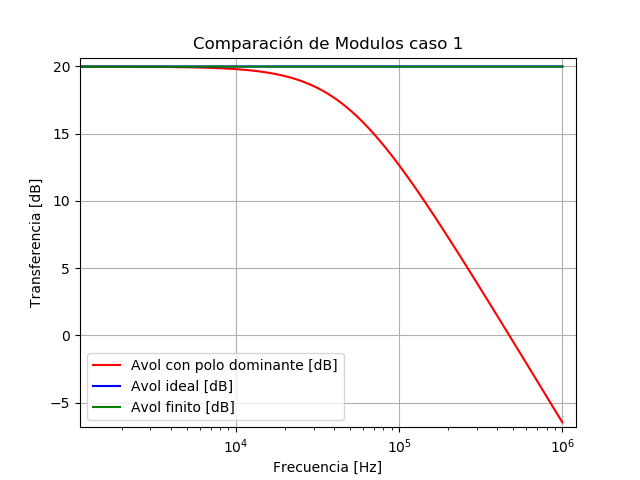
\includegraphics[width=\textwidth]{Ejercicio1/Imagenes/HCompC1.png}
	\caption{$A_{Vol}(\omega)$ Caso 1.}
	\label{fig:AvolC1}
\end{figure}
\begin{figure}[H]	
	\centering
	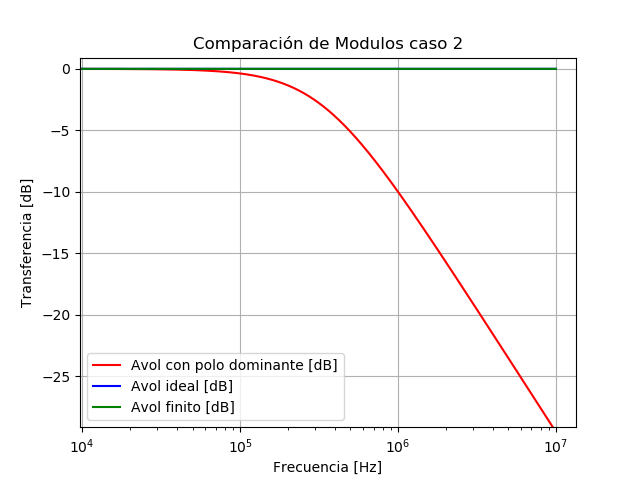
\includegraphics[width=\textwidth]{Ejercicio1/Imagenes/HCompC2.png}
	\caption{$A_{Vol}(\omega)$ Caso 2.}
	\label{fig:AvolC2}
\end{figure}
\begin{figure}[H]	
	\centering
	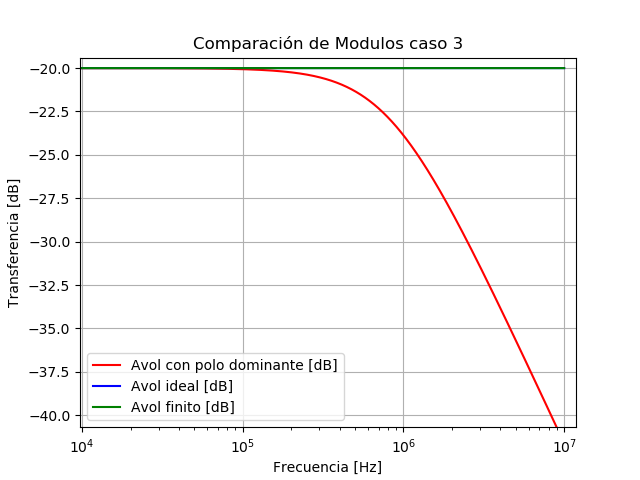
\includegraphics[width=\textwidth]{Ejercicio1/Imagenes/HCompC3.png}
	\caption{$A_{Vol}(\omega)$ Caso 3.}
	\label{fig:AvolC3}
\end{figure}

Se puede apreciar que cuanto más baja sea la ganancia, mayor será el ancho de banda, y que a partir de la frecuencia de corte cada sistema el opamp comienza a atenuar.

El error de utilizar el caso de $A_{Vol}$ ideal en lugar del caso con polo dominante se calculó como:
\begin{equation}
	Error = \frac{|A_{Vol}(\omega)-A_{Vol-Ideal}|}{A_{Vol}(\omega)}
	\label{equ:error}
\end{equation}

obteniendo los siguientes gráficos:

\begin{figure}[H]	
	\centering
	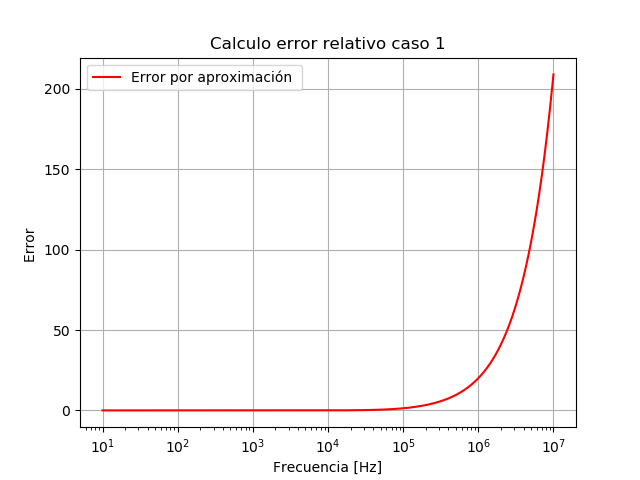
\includegraphics[width=\textwidth]{Ejercicio1/Imagenes/error1.png}
	\caption{Error relativo por aproximar Caso 1.}
	\label{fig:e1}
\end{figure}
\begin{figure}[H]	
	\centering
	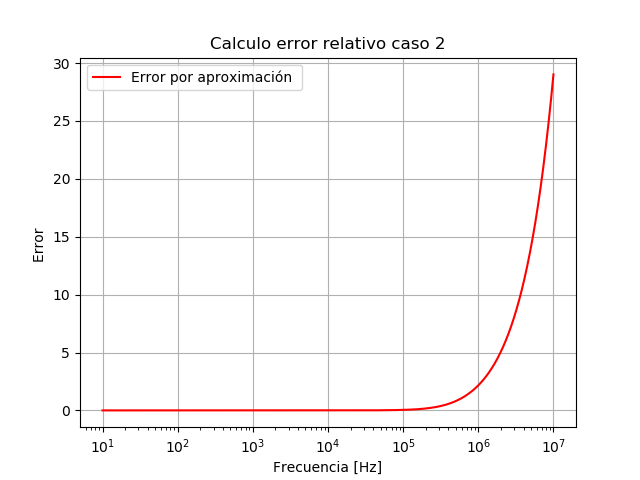
\includegraphics[width=\textwidth]{Ejercicio1/Imagenes/error2.png}
	\caption{Error relativo por aproximar Caso 2.}
	\label{fig:e2}
\end{figure}
\begin{figure}[H]	
	\centering
	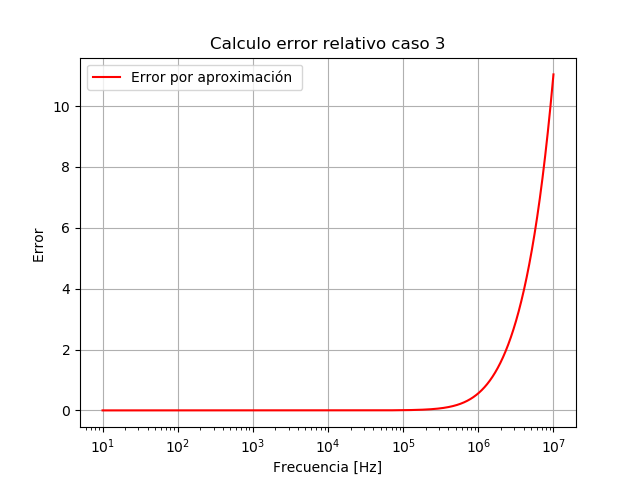
\includegraphics[width=\textwidth]{Ejercicio1/Imagenes/error3.png}
	\caption{Error relativo por aproximar Caso 3.}
	\label{fig:e3}
\end{figure}

De estos, es posible concluir que se puede utilizar la aproximación ideal siempre y cuando se tengan en cuenta la frecuencia de trabajo, y en caso de serlo necesario, el error que uno comete.

%%%%%%%%%%%%%%%%%%%%%%%%%%%%
\subsubsection{Calculo Analítico del Circuito No Inversor.}

De la misma forma que en el circuito inversor, se decidió aplicar el teorema de Thevenin.

\begin{figure}[H]
\begin{center}
\begin{circuitikz}
	\node [op amp](A1){};
	\draw (A1.-) to[short] ++(-1,0) to[R, l_=$R_1$] ++(-1.5,0) to[short] ++(-0.5,0) node[ground]{};
	\draw (A1.-) node[label=south:$V^-$]{};
	\draw (A1.+) node[label=south:$V^+$]{};
	\draw (A1.-) to[short] ++(0,1.5) to[R, l = $R_2$, i<_= $I_f$] ++(3,0) to[short] ++(0,-2);
	\draw (A1.out) to[short, -o] ++(1,0) node[ocirc,label=right:$V_{out}$]{};
	\draw (A1.+) to[short] ++(-1,0) to[R, l= $R_{Thevenin}$] ++(-1.5,0) to[short, -o] node[ocirc,label=left:$V_{Thevenin}$]{} ++(-0.5,0);
	\end{circuitikz}
	\caption{Equivalente de Thevenin del circuito inversor.}
	\label{fig:noinvThevenin}
\end{center}
\end{figure}

Siendo 
\begin{align}
	V_{Thevenin} = V_{in} \cdot \frac{R_4}{R_4+R_3} \\
	R_{Thevenin} = \frac{R_4\cdot R_3}{R_4+R_3}
\label{eq:noinvthev}
\end{align} 

Utilizando (\ref{equ:avoligualvo}) y planteando además

\begin{equation}
	V^+ = V_{Thevenin}
	\label{equ:noinvv+}
\end{equation}

\begin{equation}
	V^- = I_f R_1
\end{equation}

\begin{equation}
	V_{out} - I_f R_1 = V^-
\end{equation}

y operando algebraicamente, se puede demostrar que

\begin{equation}
	H \left(s \right) =\frac{A_{0}}{R_3} \cdot	\frac{R_3 // R_4}{1 \ + \ A_{0} \frac{R_1 // R_2}{R_2} } \cdot \left[ \frac{s}{\omega' \cdot \left( 1 + A_{0} \frac{R_1 // R_2}{R_2} \right)}  \ + \ 1 \right]^{-1}
	\label{equ:noinvtransferencia}
\end{equation}

considerando para este caso (\ref{eq:PoloDom}).

Para el caso de $A_{Vol}$ finito simplemente basta tomar:

\begin{equation}
	\lim_{\omega'\to\infty} H \left(s \right) =\frac{A_{0}}{R_3} \cdot	\frac{R_3 // R_4}{1 \ + \ A_{0} \frac{R_1 // R_2}{R_2} } \cdot \left[ \frac{s}{\omega' \cdot \left( 1 + A_{0} \frac{R_1 // R_2}{R_2} \right)}  \ + \ 1 \right]^{-1}
\end{equation}

Resultando en:

\begin{equation}
	H_{A_{vol}\space fin}\left(s \right) =\frac{A_{0}}{R_3} \cdot	\frac{R_3 // R_4}{1 \ + \ A_{0} \frac{R_1 // R_2}{R_2} }
	\label{equ:noinvtransferencia_avolfinito}
\end{equation}

Por otro lado, para $A_{Vol}$ finito solamente basta tomar:

\begin{align}
	\lim_{A_{vol}\to\infty} H_{A_{vol}=\infty} \left(s \right) = \frac{R_3 // R_4}{R_3} \cdot \frac{R_2}{R_1 // R_2}
\end{align}

Resultando en:

\begin{align}
	H_{A_{vol}=\infty} \left(s \right) = \frac{R_3 // R_4}{R_3} \cdot \frac{R_2}{R_1 // R_2}
		\label{equ:noinvtransferencia_ideal}
\end{align}

De (\ref{equ:noinvtransferencia}) se tiene que

\begin{equation}
	f_c = \frac{\omega'}{2 \pi}\cdot \left( 1 + A_{0} \frac{R_1 // R_2}{R_2} \right)
\end{equation}

Reemplazando con los valores presentados en la Tabla (\ref{tabla:resasignadas}), se puede recrear la Tabla (\ref{tabla:gananciasinv}) para el caso del circuito no inversor.

\begin{table}[H]
\begin{center}
\begin{tabular}{|c|c|c|c|}
\hline
\textbf{Caso}            & \textbf{1} & \textbf{2} & \textbf{3} \\ \hline
\textbf{$H(s)_{\infty}$} & $8.8$         & $1.6$          & $0.88$        \\ \hline
\textbf{$H(s)_{Finito}$} & $8.8$     & $1.6$     & $0.88$     \\ \hline
\textbf{$f_c$}           & $90.92 \ kHz$   & $500.01 \ kHz$  & $909.1 \ kHz$     \\ \hline
\end{tabular}
\caption{Ganancias y frecuencias de corte de los circuitos no inversores.}
\end{center}
\end{table}

De esta forma, se procede a comparar la transferencia para cada una de las consideraciones tenias en cuenta.

\begin{figure}[H]	
	\centering
	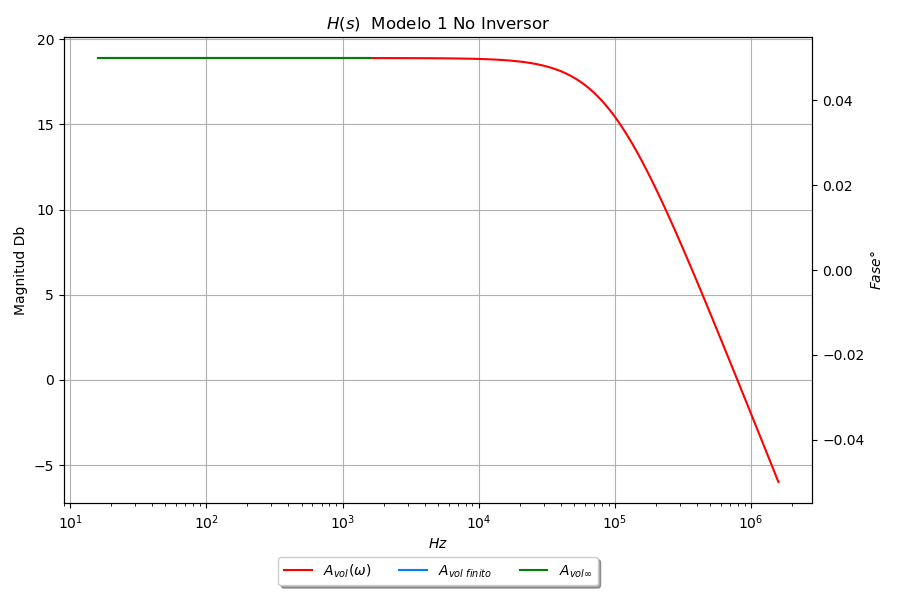
\includegraphics[width=\textwidth, trim = {0 0 2.2cm 0},clip]{Ejercicio1/Imagenes/HCompC1_noinv.png}
	\caption{$H(s)$ para el Caso 1.}
	\label{fig:AvolC1_noinv}
\end{figure}

\begin{figure}[H]	
	\centering
	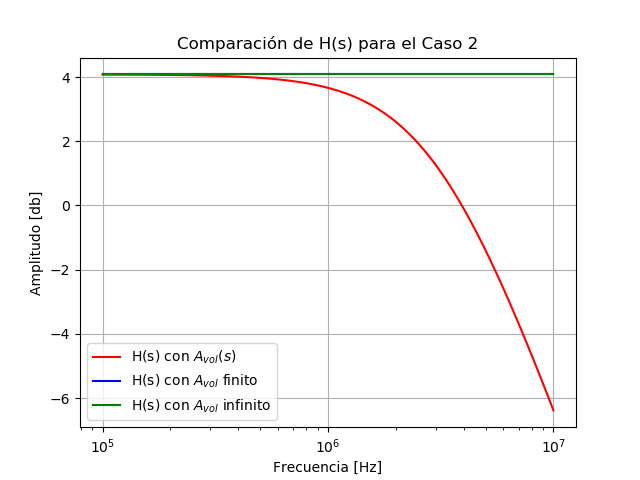
\includegraphics[width=\textwidth, trim = {0 0 2.2cm 0},clip]{Ejercicio1/Imagenes/HCompC2_noinv.png}
	\caption{$H(s)$ para el Caso 2.}
	\label{fig:AvolC2_noinv}
\end{figure}

\begin{figure}[H]	
	\centering
	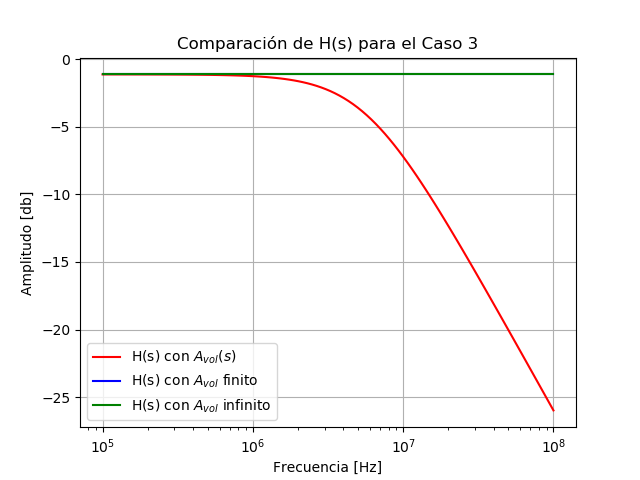
\includegraphics[width=\textwidth, trim = {0 0 2.1cm 0},clip]{Ejercicio1/Imagenes/HCompC3_noinv.png}
	\caption{$H(s)$ para el Caso 3.}
	\label{fig:AvolC3_noinv}
\end{figure}

%De igual forma que se realizó con el circuito inversor, se emplea (\ref{equ:error}) para calcular el error al considerar $A_{vol} (s)$ frente a $A_{vol \infty}$.
%
%\begin{figure}[H]	
%	\centering
%	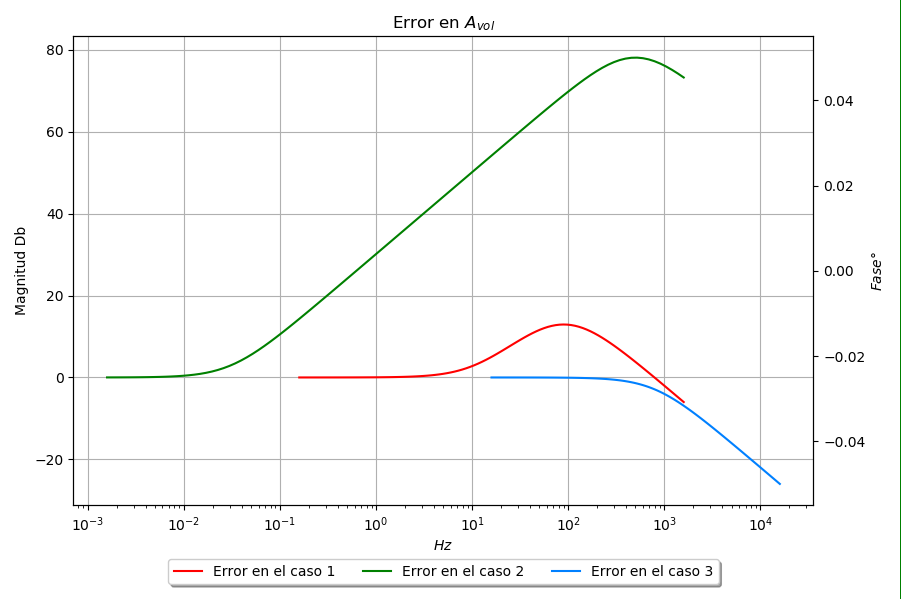
\includegraphics[width=\textwidth]{Ejercicio1/Imagenes/errornoinv.png}
%	\caption{Error relativo por aproximar $A_{vol}(s)$ para los distintos casos.}
%	\label{fig:enoinv}
%\end{figure}

%%%%%%%%%%%%%%%%%%%%%%%%%%%%%%%%%%%%%%%%%%
\subsubsection{Impedancia de entrada.}

Para calcular la impedancia de entrada de los casos presentados se sigue la misma idea de la primer parte.

Se procede a analizar el caso del inversor. Sabiendo que
\begin{align}
\label{eq:Zin}
\frac{V_{Th} - V^-}{R_{Th}}=I_{in}
\end{align}
y ademas, utilizando (\ref{eq:thev}), (\ref{eq:nodeInv}) y (\ref{eq:Vout}), se puede llegar a la siguiente expresión:
\begin{align}
	Z_{in}(s)=\frac{A_{Vol}R_1R_3+R_1R_2+R_2R_3+R_1R_3}{A_{Vol}R_3+R_2+R_3}\cdot \frac{1+\frac{s\cdot (R_1R_2+R_1R_3+R_2R_3)}{\omega ' \cdot (A_{Vol}R_1R_3+R_1R_2+R_1R_3+R_2R_3)}}{1+\frac{s\cdot (R_2+R_3)}{\omega ' \cdot(A_{Vol}R_3+R_2+R_3)}}
\end{align}

También se puede observar en (\ref{eq:Zin}) que si $A_{Vol}$ es infinito, se cumple
\begin{align} V^- = V^+=0 \implies Z_{in}=R_1
\end{align}

Por otro lado, planteando de forma similar para el no inversor:
\begin{align}
\label{eq:noinvZin}
\frac{V_{Th} - V^+}{R_{Th}}=I_{in}
\end{align}
y valiendose del uso de (\ref{equ:noinvv+}), se llega a

\begin{equation}
	Z_{in} = R_3 + R_4
	\label{equ:zinnoinv}
\end{equation}

Las mediciones de la impedancia de entrada se realizaron de la siguiente manera:

\begin{center}
\begin{circuitikz}[american voltages] \draw (0,0)
  node[draw,minimum width=2cm,minimum height=2.4cm] (load) {Load}
  ($(load.west)!0.75!(load.north west)$) coordinate (la)
  ($(load.west)!0.75!(load.south west)$) coordinate (lb)
  (lb) to[short,-o] ++(-0.5,0) coordinate (b) node[ground]{}
  to[short] ++(-4,0) coordinate (VThb);
  \draw (VThb |- la) to[sV, v_=$V_{In}$] (VThb);
  \draw (VThb |- la)
  to[R=$R$] ++(2.5,0) coordinate (VTht)
  to[short,-o,i=$I_{In}$] (VTht -| b) coordinate (a) node[above] {$A$}
  to[short] (la);
  \path (a) node[below] {$+$} -- node {$V$} (b) node[above] {$\vphantom{+}-$};
\end{circuitikz}
\end{center}

Se optó por medir la de entrada la señal y la existente en el punto A, para poder emplear la de resta de ellas mediante el modo ``math'' del osciloscopio. Luego, se observó la proporción en decibeles y la fase, tanto de la resta como de la entrada, obteniendo las medidas correspondientes a la siguiente expresión:
\begin{align}
20\log\left(\frac{V_{(A-In)}}{V_{in}}\right)
\end{align}

A partir de estos valores se puede obtener la impedancia de entrada de la forma:

\begin{align}
Z_{In}=20\log\left(\frac{V_{In}}{I_{in}}\right) =20\log\left(\frac{V_{In} \cdot  R}{V_{(A-In)}}\right) = -20\log\left(\frac{V_{(A-In)}}{V_{In} }\right)+20\log (R)
\end{align}
para la fase con medir simplemente con medir la diferencia de fase entre la señal de entrada y la que cae sobre la resistencia es equivalente a medir la de la corriente  de entrada y la tensión de entrada dado a que la corriente sobre la resistencia y la caida de tensión sobre ella tienen la misma fase.


Luego se realizaron mediciones de la impedancia de entrada. De esta forma se compararon con simulaciones realizadas en LTSpice y con el calculo analítico. Cabe aclarar que para los gráficos, al realizar el calculo analítico, no fueron tomadas en cuentas las puntas del osciloscopio, las cuales se emplearon en modo \textbf{x1}, de forma que alteraron la medición, mientras que en las simulaciones con LTSpice si fueron tomadas en cuenta.

A continuación se presentan dichas medidas para el circuito inversor.

\begin{figure}[H]	
	\centering
	
\includegraphics[width=0.9\textwidth]{Ejercicio1/Imagenes/ZinC1.png}
	\caption{BODE en modulo para el Caso 1 del circuito inversor.}
	\label{fig:CompZinC1inv}
\end{figure} 

\begin{figure}[H]	
	\centering
	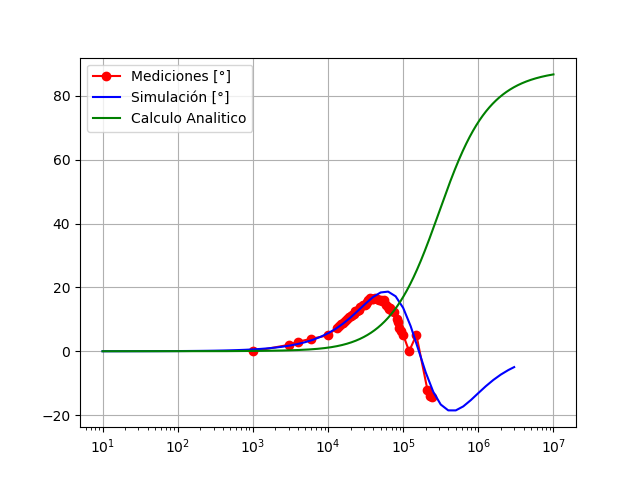
\includegraphics[width=0.9\textwidth]{Ejercicio1/Imagenes/ZinphC1.png}
	\caption{BODE en fase para el Caso 1 del circuito inversor.}
	\label{fig:CompZinphC1inv}
\end{figure} 

\begin{figure}[H]	
	\centering
	
\includegraphics[width=0.9\textwidth]{Ejercicio1/Imagenes/CZinC2.png}
	\caption{BODE en modulo para el Caso 2 del circuito inversor.}
	\label{fig:CompZinC2inv}
\end{figure} 

\begin{figure}[H]	
	\centering
	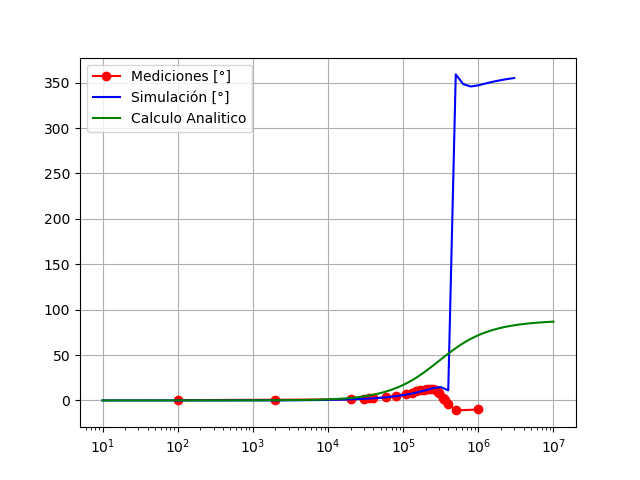
\includegraphics[width=0.9\textwidth]{Ejercicio1/Imagenes/ZinphC2.png}
	\caption{BODE en fase para el Caso 2 del circuito inversor.}
	\label{fig:CompZinphC2inv}
\end{figure} 

\begin{figure}[H]	
	\centering
	
\includegraphics[width=\textwidth]{Ejercicio1/Imagenes/CZinC3.png}
	\caption{BODE en modulo para el Caso 3 del circuito inversor.}
	\label{fig:CompZinC3inv}
\end{figure} 

\begin{figure}[H]	
	\centering
	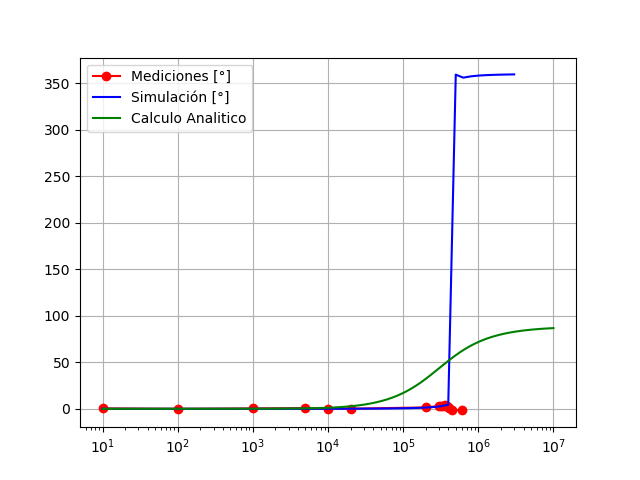
\includegraphics[width=\textwidth]{Ejercicio1/Imagenes/ZinphC3.png}
	\caption{BODE en fase para el Caso 3 del circuito inversor.}
	\label{fig:CompZinphC3inv}
\end{figure}

También cabe destacar que en las Figuras (\ref{fig:CompZinphC2inv}) y (\ref{fig:CompZinphC3inv}) realmente no hay un salto, sino que es un cambio de fase de $360^{\circ}$.

Luego se procede a mostrar las mediciones realizadas para el caso del circuito no inversor.

\begin{figure}[H]	
	\centering
	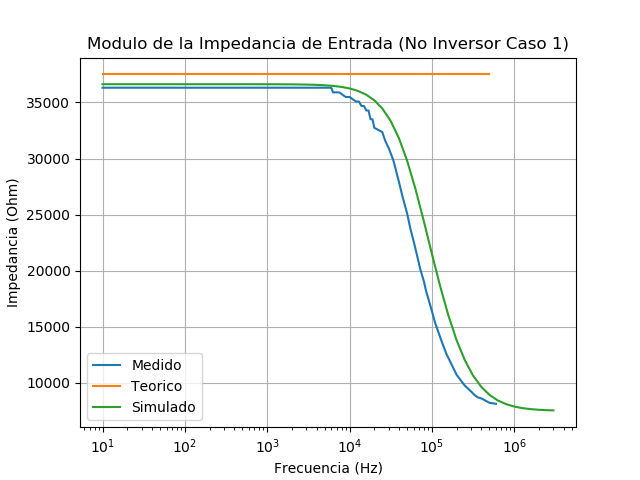
\includegraphics[width=0.9\textwidth]{Ejercicio1/Imagenes/ZinC1_Noinv.png}
	\caption{BODE en modulo para el Caso 1 del circuito no inversor.}
	\label{fig:NoInvCompZinC1}
\end{figure} 

\begin{figure}[H]	
	\centering
	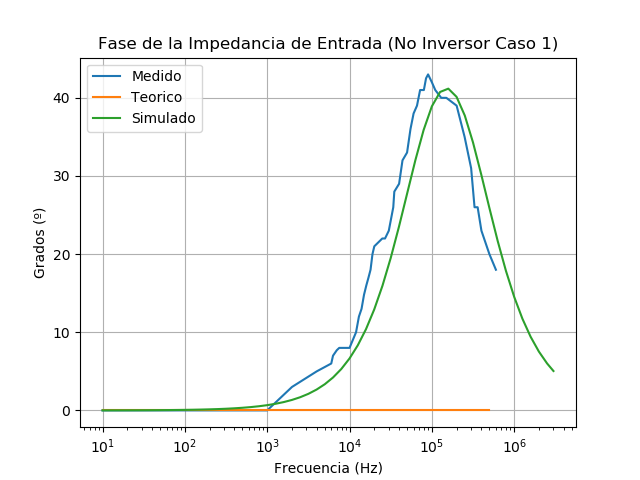
\includegraphics[width=0.9\textwidth]{Ejercicio1/Imagenes/ZinphC1_Noinv.png}
	\caption{BODE en fase para el Caso 1 del circuito no inversor.}
	\label{fig:NoInvCompZinphC1}
\end{figure} 

\begin{figure}[H]	
	\centering
	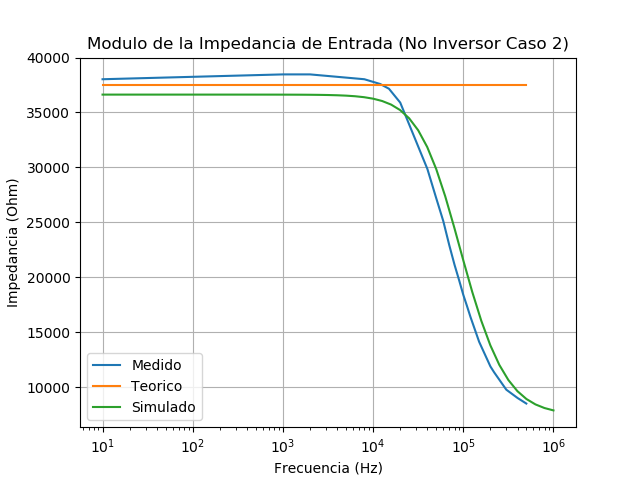
\includegraphics[width=0.9\textwidth]{Ejercicio1/Imagenes/ZinC2_Noinv.png}
	\caption{BODE en modulo para el Caso 2 del circuito no inversor.}
	\label{fig:NoInvCompZinC2}
\end{figure} 

\begin{figure}[H]	
	\centering
	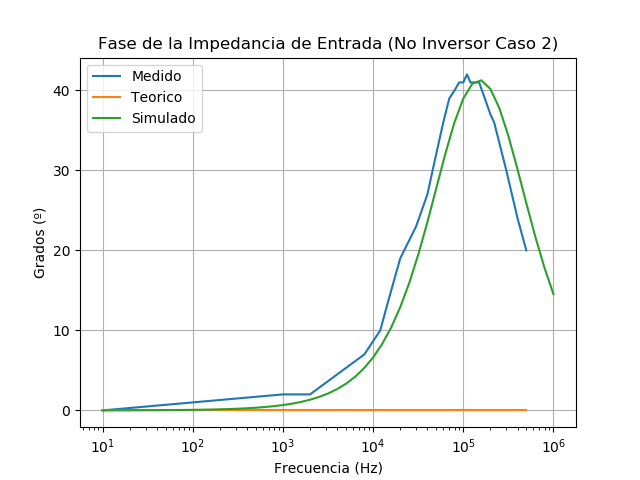
\includegraphics[width=0.9\textwidth]{Ejercicio1/Imagenes/ZinphC2_Noinv.png}
	\caption{BODE en fase para el Caso 2 del circuito no inversor.}
	\label{fig:NoInvCompZinphC2}
\end{figure} 

\begin{figure}[H]	
	\centering
	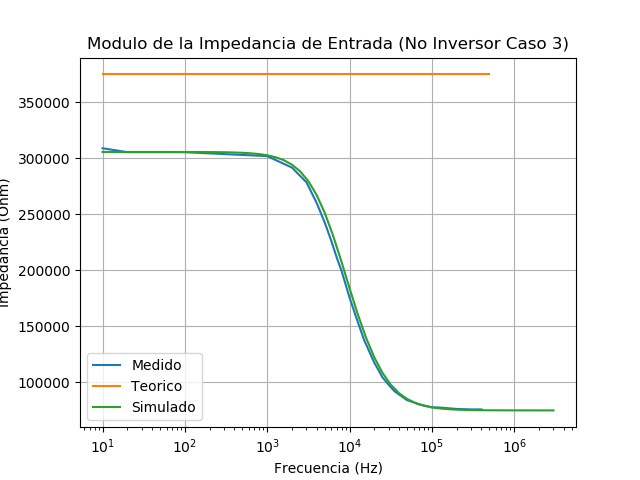
\includegraphics[width=\textwidth]{Ejercicio1/Imagenes/ZinC3_Noinv.png}
	\caption{BODE en modulo para el Caso 3 del circuito no inversor.}
	\label{fig:NoInvCompZinC3}
\end{figure} 

\begin{figure}[H]	
	\centering
	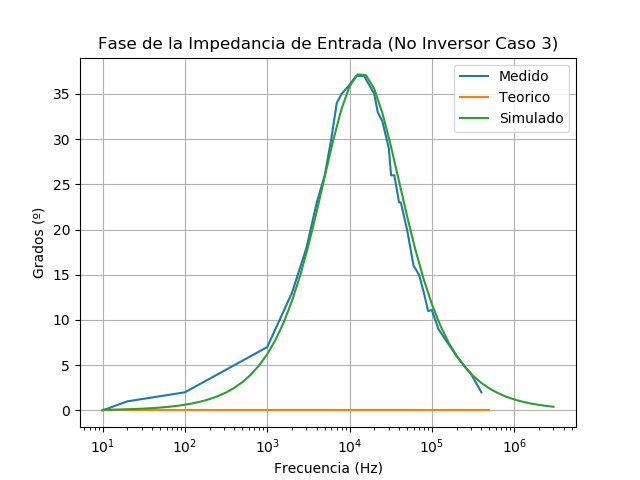
\includegraphics[width=\textwidth]{Ejercicio1/Imagenes/ZinphC3_Noinv.png}
	\caption{BODE en fase para el Caso 3 del circuito no inversor.}
	\label{fig:CompZinphC3}
\end{figure}

%%%%%%%%%%%%%%%%%%%%%%%%%%%%%%
\subsubsection{Máximos valores de entrada.}

\begin{center}
\textcolor{red}{\textbf{VER PARA EL NO INVERSOR.}}
\textcolor{red}{\textbf{HACER LAS CUENTAS Y LOS GRÁFICOS.}}
\end{center}

El máximo valor de entrada a partir del cual el opamp satura se encuentra definido por diversas variables, siendo algunas de ellas la ganancia del sistema, la amplitud y la frecuencia de la entrada.

Al momento de definir los valores posibles, se realizó un enfoque en las tres variables previamente mencionadas y se asumió el opamp con ganancia ideal. Cabe recordar que se empleó la formula $ V_{Out}=H(s)\cdot V_{in} $.

De esta forma, el máximo valor de $V_{in}$ queda definido por la tensión de saturación del operacional. Para el utilizado en este informe (LM324), dicho valor es de $Vcc - 1.5 \ V$\footnote{Dato extraído de la hoja de datos.}, siendo así, para el caso empleado, equivalente a $13.5 \ V$. Luego, utilizando esta relación, se plasmaron los resultados, para las distintas ganancias analizadas, en la Tabla (\ref{tab:gananciaideal}). Cabe descara que para el caso 3 se realiza una excepción, ya que el fabricante informa que la máxima tensión de entrada soportada por el dispositivo sin quemarse es de $32 \ V$.

\begin{table}[H]
\begin{center}
\label{tab:maxin}
\begin{tabular}{|c|c|c|c|}
\hline
\textbf{Caso}        & \textbf{1} & \textbf{2} & \textbf{3} \\ \hline
\textbf{Ganancia ideal}     & 10         & 1          & 0.1        \\ \hline
\textbf{$V_{in-Max} \ \left[ V \right]$} & 1.35       & 13.5       & 32         \\ \hline
\end{tabular}
\end{center}
\caption{Ganancia ideal para el operacional LM324.}
\label{tab:gananciaideal}
\end{table}

Luego se graficó la máxima tensión de entrada en función de la ganancia:
\begin{figure}[H]	
	\centering
	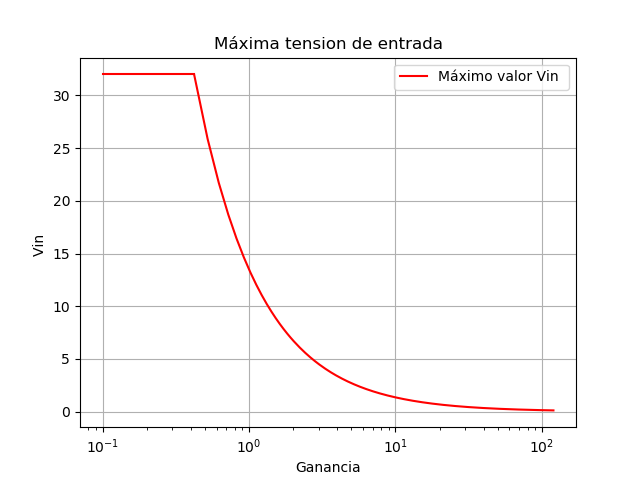
\includegraphics[width=\textwidth]{Ejercicio1/Imagenes/maxvin.png}
	\caption{Máxima tensión de entrada en función de la ganancia.}
	\label{fig:MaxVin}
\end{figure} 

También se analizó la máxima amplitud de entrada en función de la frecuencia tal que no haya Slew-Rate, el cual es un efecto que se detalla con mayor profundidad en su propia sección, ni saturación.
La cual puede ser apreciada en el siguiente gráfico:
\begin{figure}[H]	
	\centering
	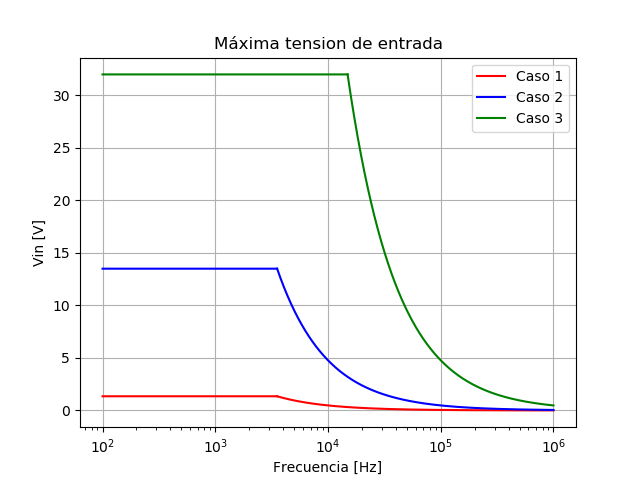
\includegraphics[width=\textwidth]{Ejercicio1/Imagenes/maxvinsr.png}
	\caption{Máxima tensión de entrada sin saturación ni Slew-Rate.}
	\label{fig:MaxVinsr}
\end{figure} 
%%%%%%%%%%%%%%%%%%
\subsubsection{Principales Características.}
En el caso del circuito inversor, considerando la situación en la cual $R_3$ sea igual a 0, la salida del amplificador operacional debería ser de $0 \ V$. Esto no es lo que ocurre dado que existe una tensión de offset, la cual se analiza en la sección 3 de este informe.

Por su parte, para el circuito no inversor,
%si se calcula nuevamente (\ref{equ:noinvtransferencia}), se obtiene
%\[
%	H \left( s \right) = \frac{1}{\frac{R_1}{R_1 + R_2} + \frac{1}{A_o \left( \omega \right)}}
%\]
se obtendría que $V^+ = V_{in}$. Este circuito se caracteriza por poder ser sustentado con una sola fuente de alimentación, siendo esta referenciada a $V^+/2$ \footnote{Caracterización brindada por el fabricante.}. Es así que recalculando la ganancia para esta disposición, se obtiene que 
\[
	H \left(s \right) = \left( \frac{R_1}{R_1 + R_2} + A_o\left( \omega \right) \right)^{-1}
\]

Luego, se sabe que $R_3$ no es necesaria considerando $I_{in}$ constante frente a cambios en la temperatura\footnote{Dato obtenido de la hoja de datos}.

\begin{figure}[H]	
	\centering
	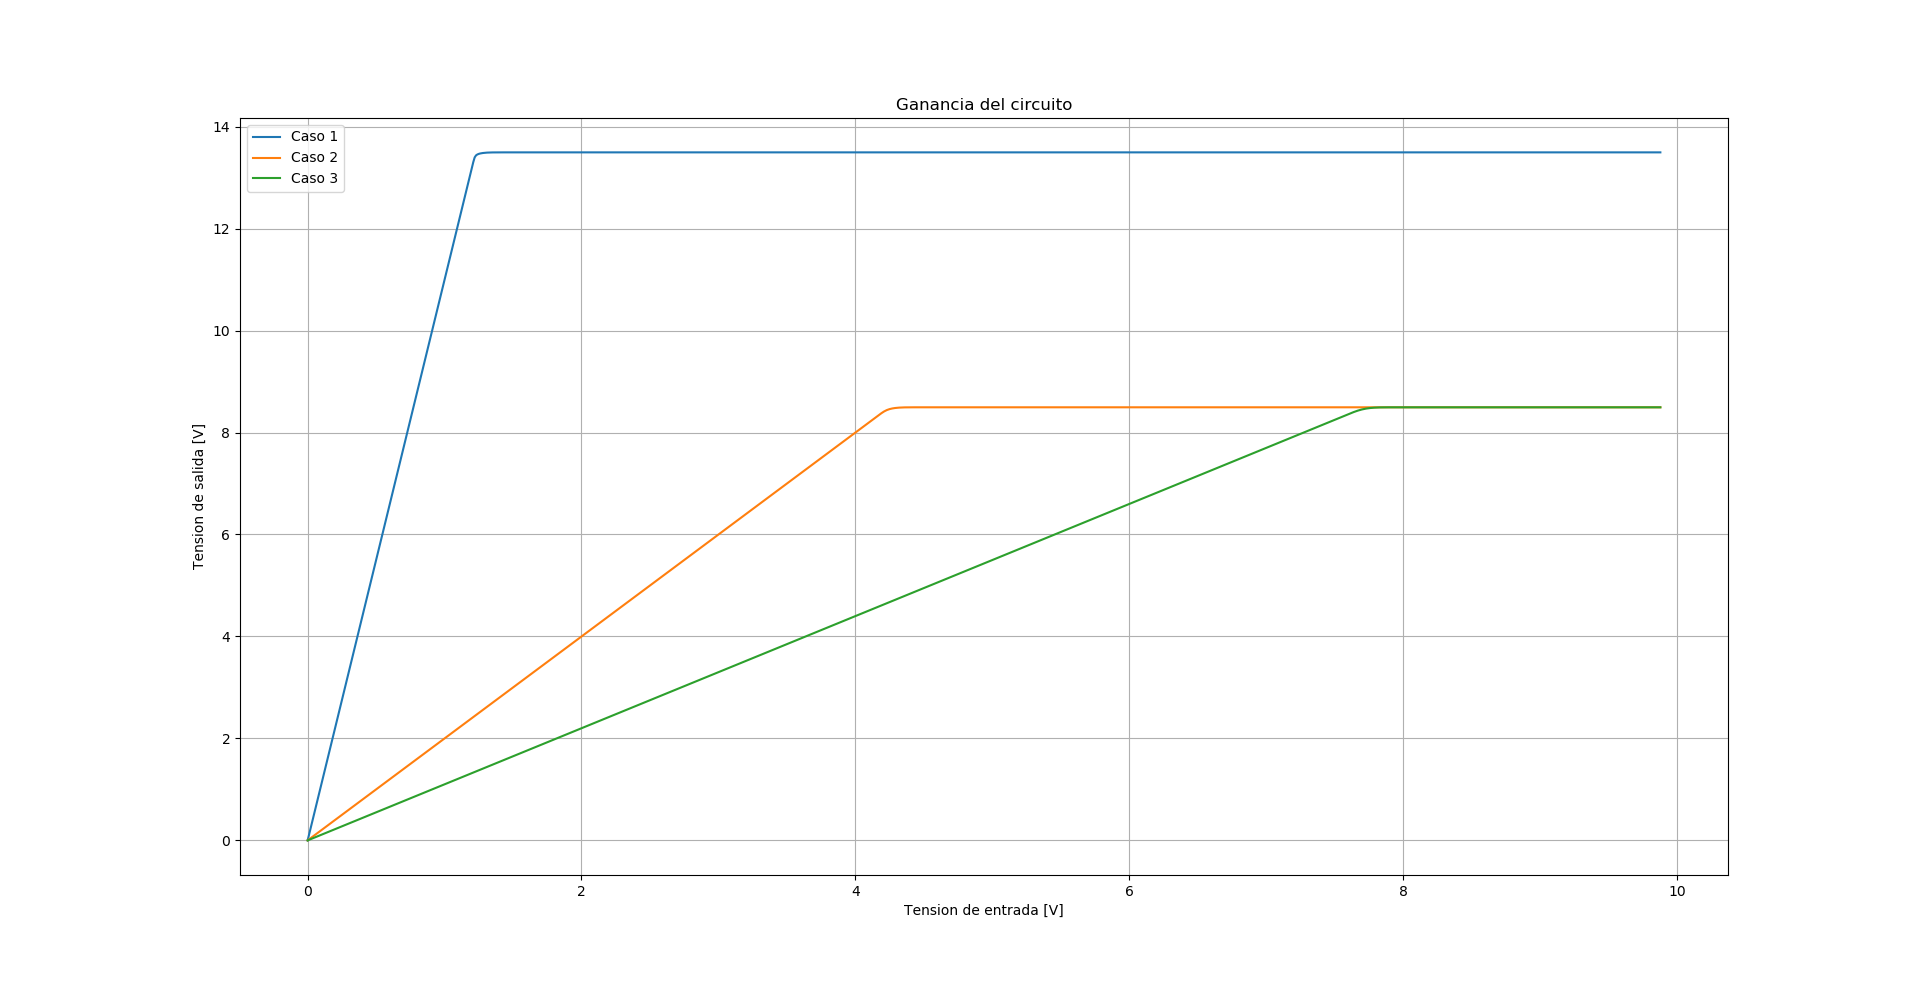
\includegraphics[width=\textwidth]{Ejercicio1/Imagenes/VinvsVoR3.png}
	\caption{$V_{out}$ en función de $V_{in}$ con $R_3 = 0 \ \Omega$ con $A_{vol \infty}$.}
	\label{fig:VinvsVoR3}
\end{figure} 

Es así que la transferencia del circuito, mostrada en la Figura (\ref{fig:VinvsVoR3}) para cada caso, diferencia dos situaciones, una donde la relación entre la salida y la entrada es lineal, con una pendiente de $1 + \frac{R_2}{R_1}$ en el caso ideal, por lo visto en (\ref{equ:noinvtransferencia_ideal}), y otra zona donde la tensión es constante debido a la saturación propia del operacional.

Además, se observa en (\ref{equ:zinnoinv}) que la impedancia de entrada decae, lo cual puede llegar a provocar que esta sea comparable con la de la fuente, generando problemas de medición.

Por otro lado, se analiza el propósito de $R_4$ en el circuito inversor. A primera vista no es evidente, dado que la transferencia es independiente de ella, pero observando que existe una corriente máxima\footnote{Dato obtenido de la datasheet, $I_{Max}=20 \ mA$} que puede aportar el opamp, se llego a que el propósito de $R_4$ es limitar la corriente, por lo tanto su valor debe ser $R_4>\frac{V_{Out}}{I_{Max}}$. Otra función que posee $R_4$ es el limitar la corriente del lazo.
%%%%%%%%%%%%%%%%%%%%

\subsubsection{DC-Sweep.}
Se realizó un barrido entre $-Vcc$ y $Vcc$, utilizando un generador de funciones con una rampa y un circuito inversor para llegar a la tensión de salida necesitada, dado que el generador de funciones solo puede entregar hasta $20 \ Vpp$.
El comportamiento del operacional no es lineal para todo el rango de entradas. Este se puede observar únicamente en el rango entre $-V_{sat}$ y $V_{sat}$. Considerando las tensiones de entrada máxima que se observan en la Figura (\ref{fig:MaxVinsr}), se registraron las siguientes mediciones para el circuito inversor:

\begin{figure}[H]	
	\centering
	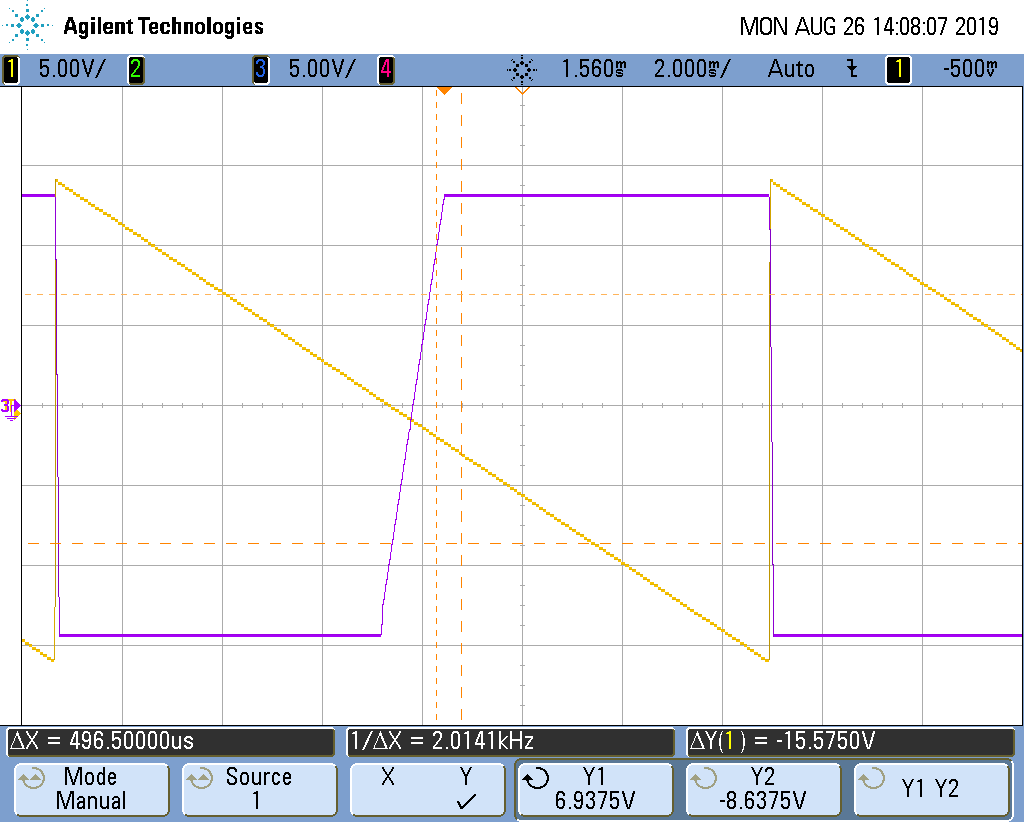
\includegraphics[width=0.8\textwidth, trim = {0 3.3cm 0 2cm},clip]{Ejercicio1/Imagenes/dc_sweep_c1.png}
	\caption{DC-sweep del circuito inversor, Caso 1.}
	\label{fig:dcc1}
\end{figure} 
Se puede observar en este caso como el opamp satura a partir de una tensión mayor a $1.35 V$ como se predijo en le punto (a).
\begin{figure}[H]	
	\centering
	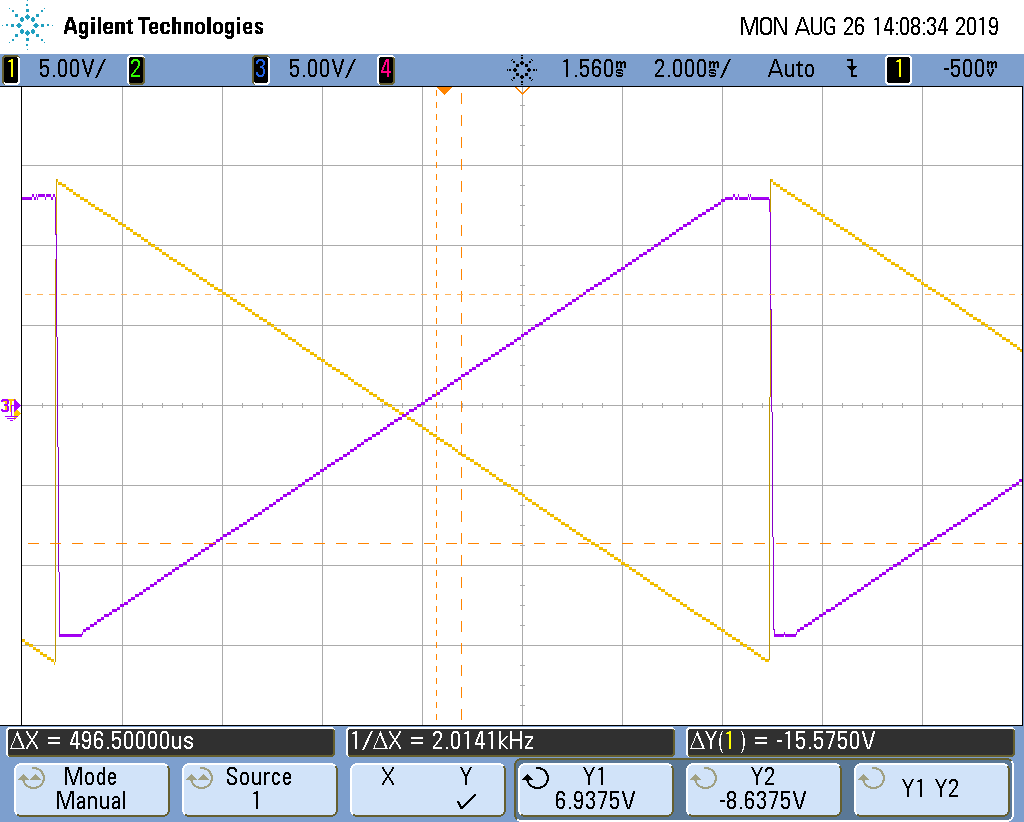
\includegraphics[width=0.8\textwidth, trim = {0 3.3cm 0 2cm},clip]{Ejercicio1/Imagenes/dc_sweep_c2.png}
	\caption{DC-sweep del circuito inversor, Caso 2.}
	\label{fig:dcc2}
\end{figure} 
En esta figura se ve como el comportamiento del amplificador operacional es lineal en la mayoría del espectro, con la excepción de las puntas, como fue explicado en el punto (a), para tensiones próximas a los $ 13.5 \ V$.
\begin{figure}[H]	
	\centering
	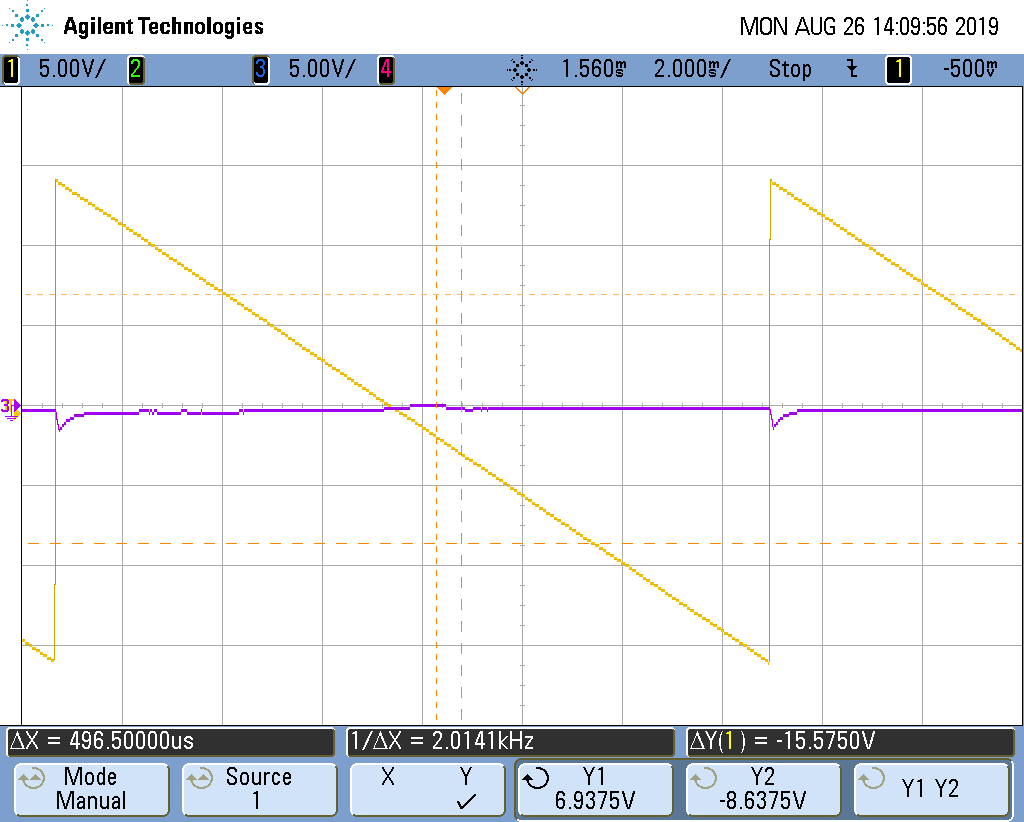
\includegraphics[width=0.8\textwidth, trim = {0 3.3cm 0 2cm},clip]{Ejercicio1/Imagenes/dc_sweep_c3.png}
	\caption{DC-sweep del circuito inversor, Caso 3.}
	\label{fig:dcc3}
\end{figure} 
Finalmente en esta figura se muestra que el opamp tiene comportamiento lineal para todos los valores de la rampa.

Luego, se procede a presentar el mismo análisis aplicado al circuito no inversor:

\begin{figure}[H]	
	\centering
	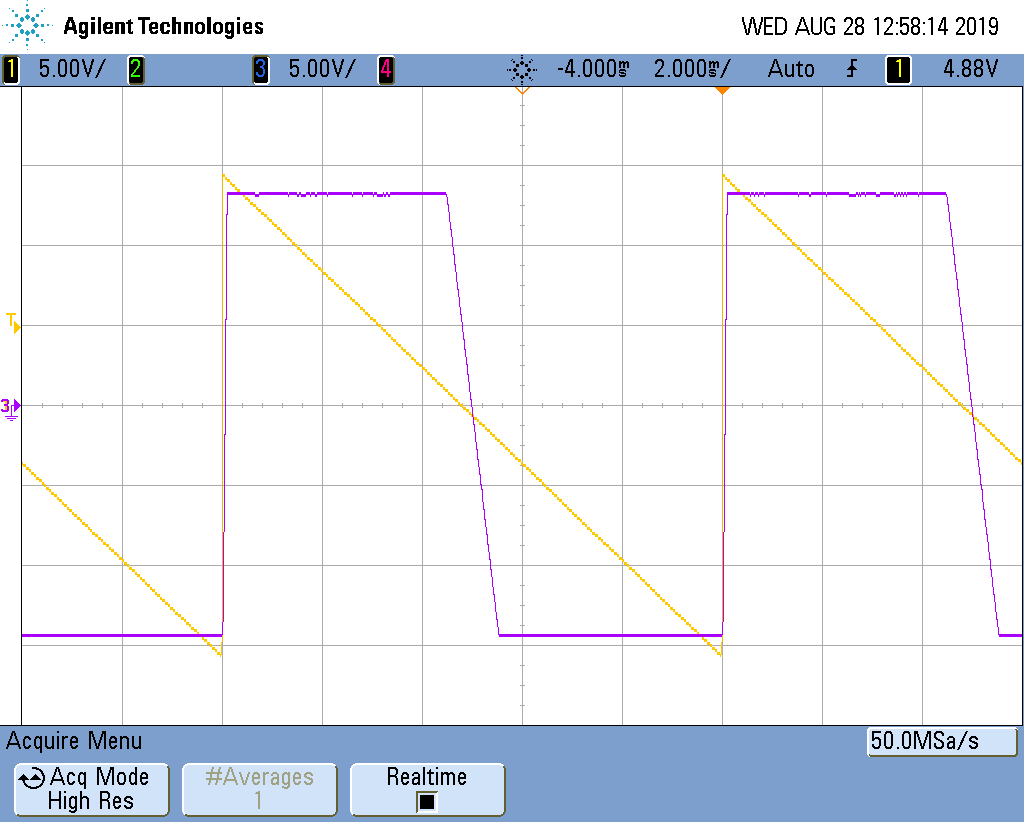
\includegraphics[width=0.8\textwidth, trim = {0 3.3cm 0 2cm},clip]{Ejercicio1/Imagenes/dc_sweep_c1_noinv.png}
	%trim={<left> <lower> <right> <upper>}
	\caption{DC-sweep del circuito no inversor, Caso 1.}
	\label{fig:dcc1noi}
\end{figure} 

\begin{figure}[H]	
	\centering
	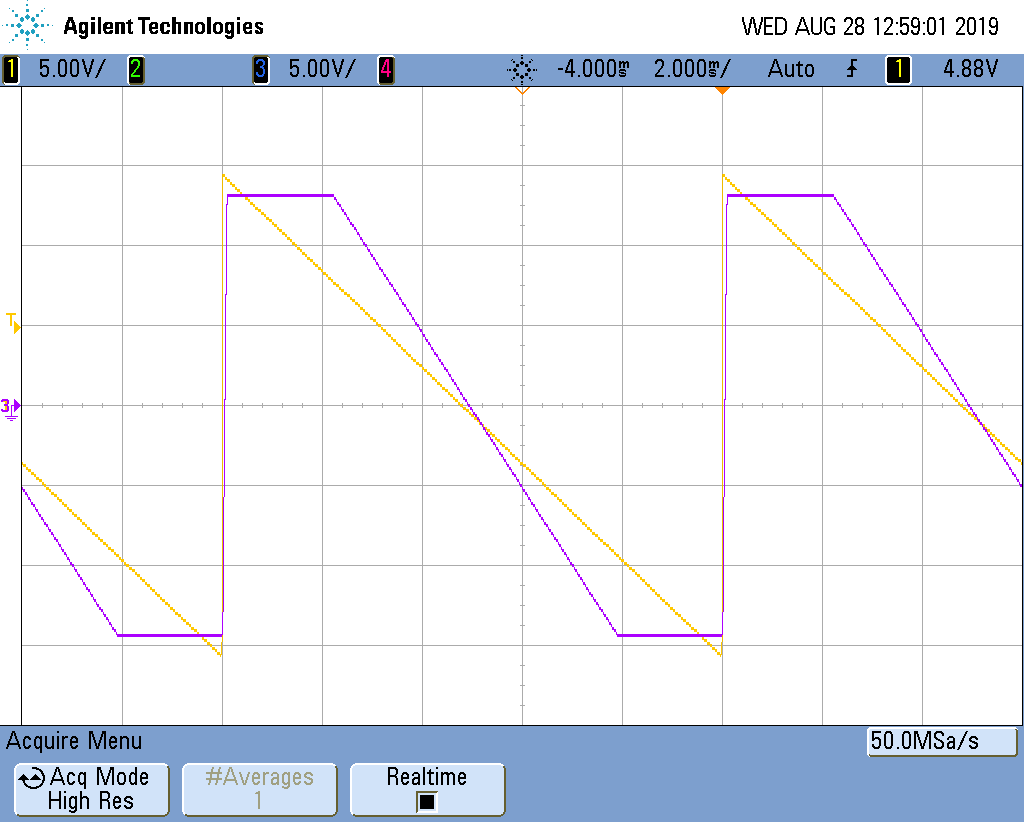
\includegraphics[width=0.8\textwidth, trim = {0 3.3cm 0 2cm},clip]{Ejercicio1/Imagenes/dc_sweep_c2_noinv.png}
	\caption{DC-sweep del circuito no inversor, Caso 2.}
	\label{fig:dcc2noi}
\end{figure} 

\begin{figure}[H]	
	\centering
	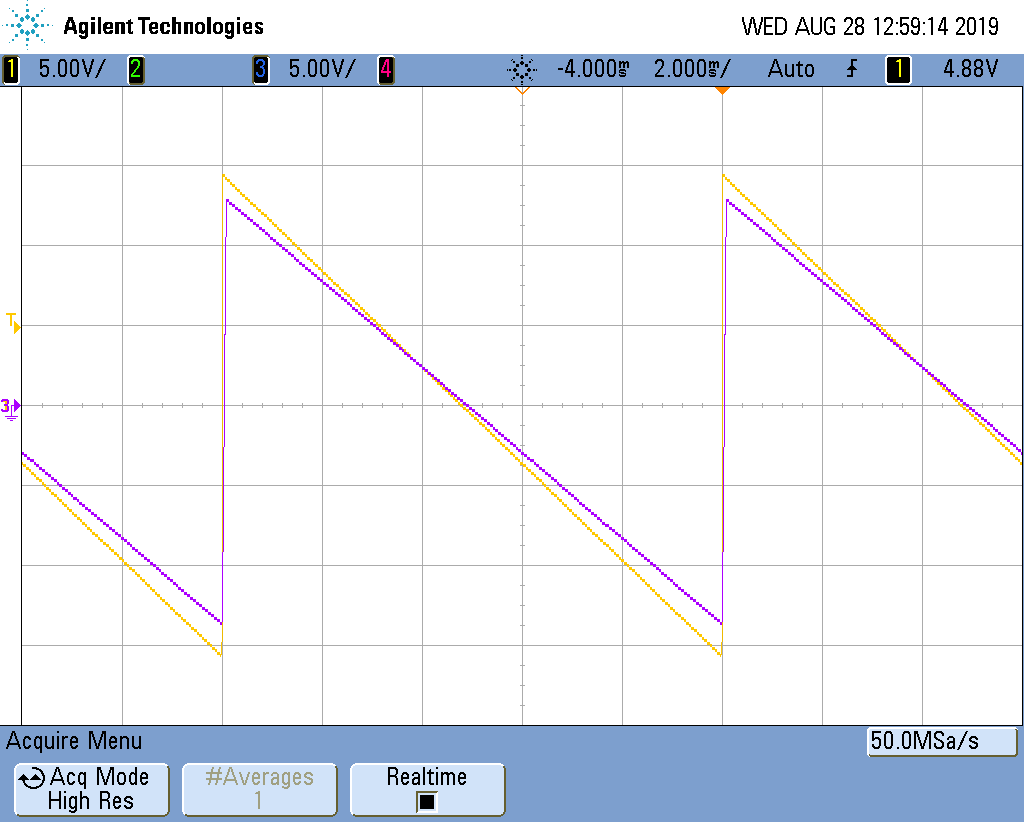
\includegraphics[width=0.8\textwidth, trim = {0 3.3cm 0 2cm},clip]{Ejercicio1/Imagenes/dc_sweep_c3_noinv.png}
	\caption{DC-sweep del circuito no inversor, Caso 3.}
	\label{fig:dcc3noi}
\end{figure} 

Los casos mostrados en las Figuras (\ref{fig:dcc1noi}), (\ref{fig:dcc2noi}) y (\ref{fig:dcc3noi}) son muy similares a los presentados en (\ref{fig:dcc1}), (\ref{fig:dcc2}) y (\ref{fig:dcc3}). Esto es un resultado esperable, ya que los ordenes con los cuales se amplifican las señales de entrada, para cada caso, son similares, provocando que las tensiones de saturación también lo sean, con la salvedad del cambio de signo en la tensión de entrada para cada tipo de circuito.

Otro efecto no lineal del amplificador operacional que fue observado es el efecto de Cross-Over, el cual es introducido dado a la polarización de los transistores que tiene por dentro el operacional. Este efecto se hace notar como una deformación en forma de llanura en la transición por $0 \ V$, como se puede apreciar en la Figura (\ref{fig:co}).

Se puede evitar tener que lidiar con este problema al aplicar una tensión de offset de continua, de forma tal que se consiga polarizar los transistores. Para ello, en este informe, se emplearon valores entre $0.7 \ V$ y $1.4 \ V$. Otra alternativa es valerse de una señal con valor medio mayor a $0.7 \ V$. 
\begin{figure}[H]	
	\centering
	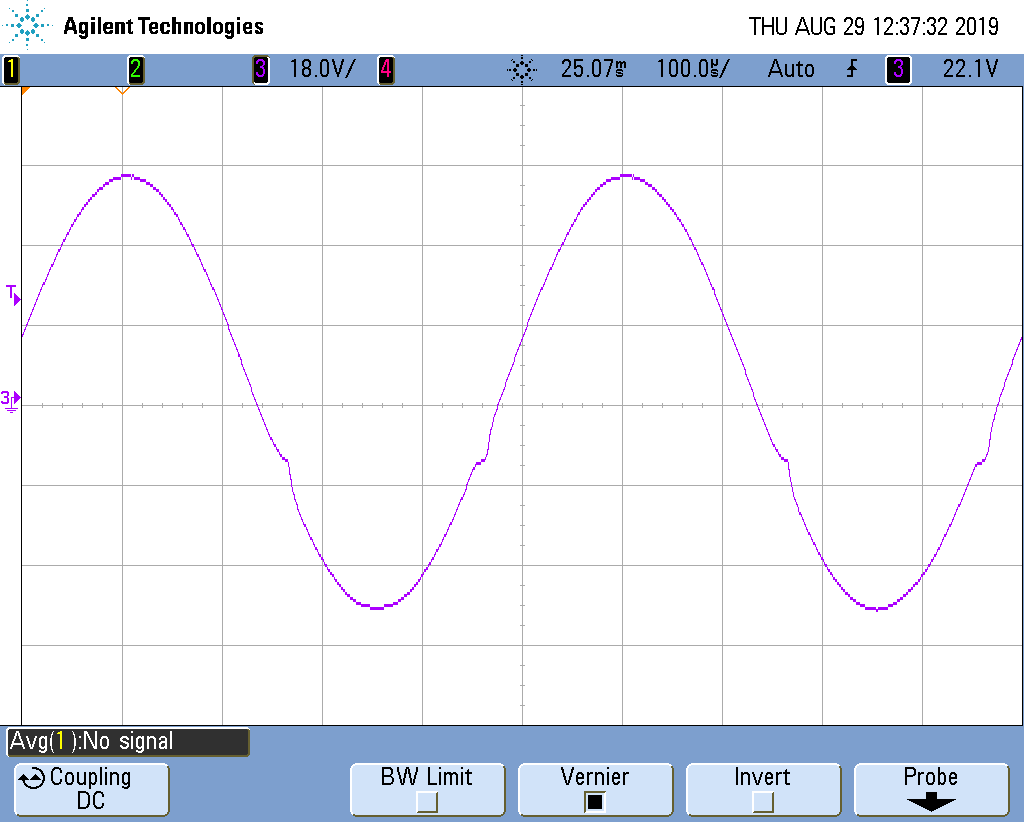
\includegraphics[width=0.8\textwidth, trim = {0 3.3cm 0 2cm},clip]{Ejercicio1/Imagenes/CrossOver.png}
	\caption{Señal con Cross-Over.}
	\label{fig:co}
\end{figure} 

%%%%%%%%%%%%%%%%%%%%%%%%%%
\subsubsection{Slew-Rate.}
El Slew-Rate está definido como la máxima variación temporal de la salida del amplificador operacional. Este efecto depende de 3 parámetros siendo estos la frecuencia, la amplitud y la ganancia, considerando el caso de que la salida sea una senoidal. Dado que se puede describir cualquier señal como una combinación lineal de senos, se puede decir que el Slew-Rate de una señal arbitraria también dependerá de estos parámetros. Si se le demanda al operacional una tasa de cambio mayor a la soportada, este procederá a distorsionar la señal.
\begin{align}
	SR= Max\left( \frac{\partial V_{Out}}{\partial t}\right)
\end{align}

Utilizando una entrada senoidal de la forma $V_{in}=A\cdot \sin (\omega t)$:
\begin{align}
	SR= Max\left( \frac{\partial (G\cdot A\cdot \sin (\omega t))}{\partial t}\right) = A \cdot \omega \cdot G  
\label{eq:sr}
\end{align}

A partir de (\ref{eq:sr}) se llega a una relación que debe cumplir la señal de entrada para no presentar efectos de Slew-Rate. Esta limitación tiene un grado de libertad, por lo tanto se puede elegir un parámetro fijo y regular el otro, por ejemplo, fijando la frecuencia de entrada, se deberá cumplir que:
\begin{align} V_{in}	\leq \frac{SR}{G\cdot \omega_0}\end{align}

Es así que se midió el Slew-Rate utilizando como entrada una senoidal, obteniendo la siguiente medición:
\begin{figure}[H]	
	\centering
	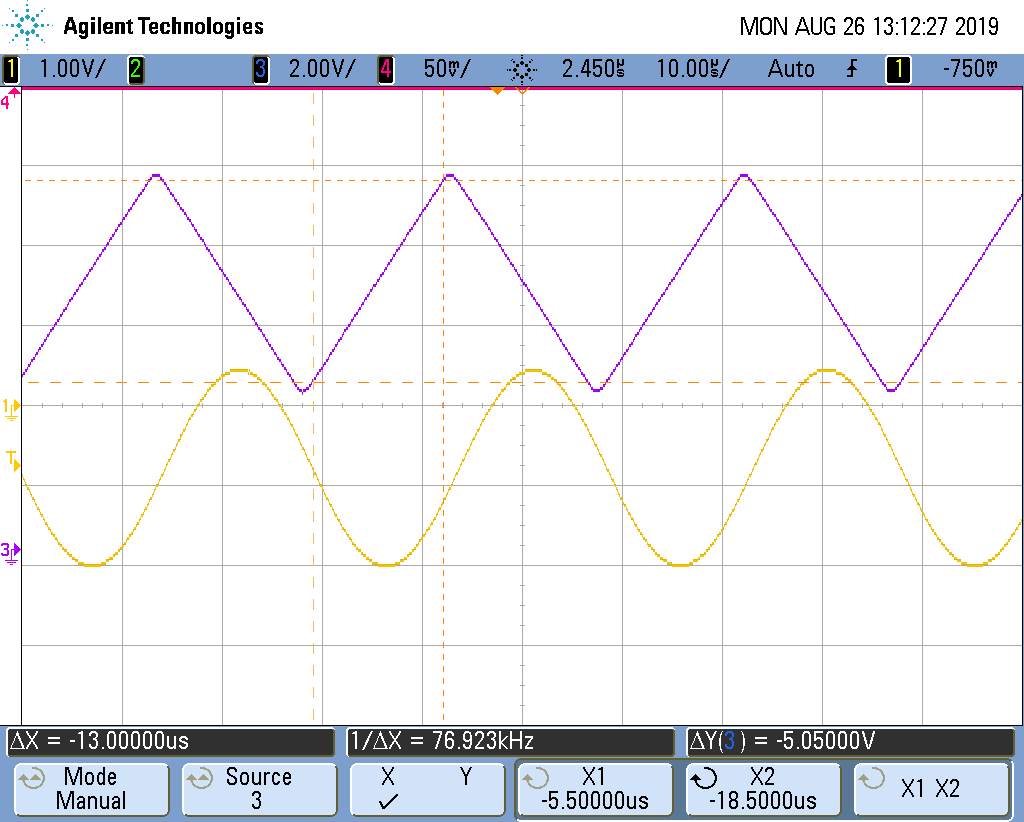
\includegraphics[width=0.8\textwidth, trim = {0 3.3cm 0 2cm},clip]{Ejercicio1/Imagenes/slew_rate1.png}
	\caption{Medición Slew-Rate.}
	\label{fig:SlewRate}
\end{figure}
De aqui utilizando (\ref{eq:sr}) se obtiene que:
\begin{align}
SR \approx  0.38 \frac{V}{\mu s}
\end{align}
lo cual concuerda con lo provisto por el fabricante en la Tabla (\ref{tab:datos}).
%%%%%%%%%%%%%%%%%%%%%%%%%%%%%%%%%%%%
\subsubsection{Respuesta en frecuencia.}
Se midió la respuesta en frecuencia de las configuraciones en los diversos casos y se graficaron junto a las simulaciones hechas en LTSpice y los cálculos teóricos.

Primero se presentan los casos para el circuito inverso.
\begin{figure}[H]	
	\centering
	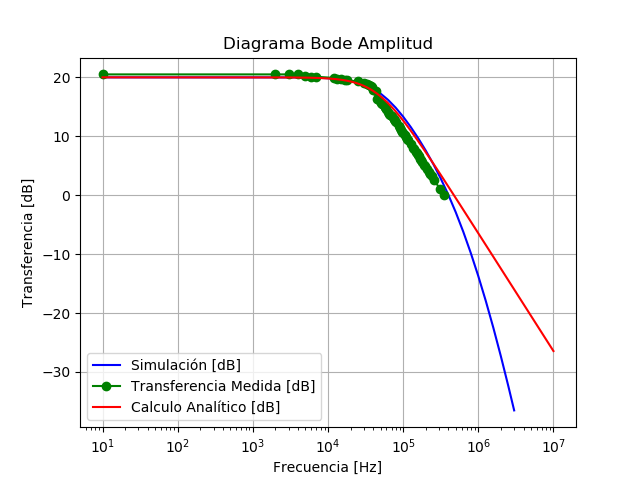
\includegraphics[width=0.8\textwidth]{Ejercicio1/Imagenes/BodeC1.png}
	\caption{Diagrama de Bode en amplitud Caso 1.}
	\label{fig:BodeC1}
\end{figure} 
\begin{figure}[H]	
	\centering
	
\includegraphics[width=0.8\textwidth]{Ejercicio1/Imagenes/BodephC1.png}
	\caption{Diagrama de Bode en fase Caso 1.}
	\label{fig:BodephC1}
\end{figure} 

En estas mediciones el principal problema que se presentó fue la saturación propia del operacional. También se evidenciaron los efectos del Slew-Rate dado a que esta configuración amplifica y efecto de Cross-Over. Además, se observó que, dado que la tensión de entrada era tan pequeña, como se puede apreciar en la Figura (\ref{fig:MaxVinsr}), la señal era comparable con ruido, el cual a su vez era amplificado y obteniendo uno mucho mayor a la salida.
\begin{figure}[H]	
	\centering
	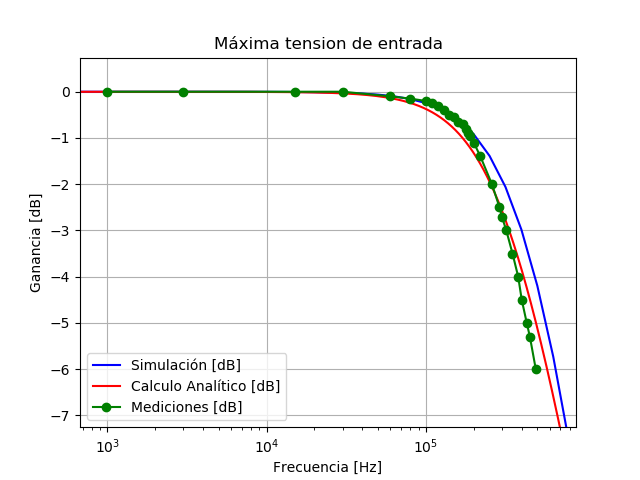
\includegraphics[width=0.8\textwidth]{Ejercicio1/Imagenes/BodeC2.png}
	\caption{Diagrama de Bode en amplitud Caso 2.}
	\label{fig:BodeC2}
\end{figure} 
\begin{figure}[H]	
	\centering
	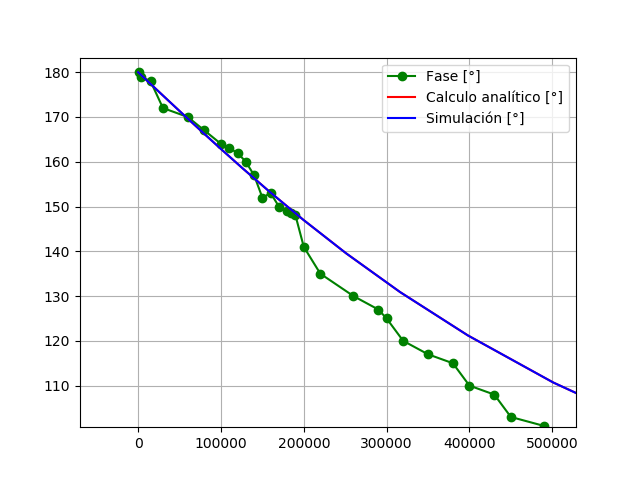
\includegraphics[width=0.8\textwidth]{Ejercicio1/Imagenes/BodephC2.png}
	\caption{Diagrama de Bode en fase Caso 2.}
	\label{fig:BodephC2}
\end{figure} 

\begin{center}
\textcolor{red}{\textbf{AQUÍ DEBERÍA DECIR ALGO ÚTIL.}}
\end{center}

\begin{figure}[H]	
	\centering
	
\includegraphics[width=0.8\textwidth]{Ejercicio1/Imagenes/BodeC3.png}
	\caption{Diagrama de Bode en amplitud Caso 3.}
	\label{fig:BodeC3}
\end{figure} 
\begin{figure}[H]	
	\centering
	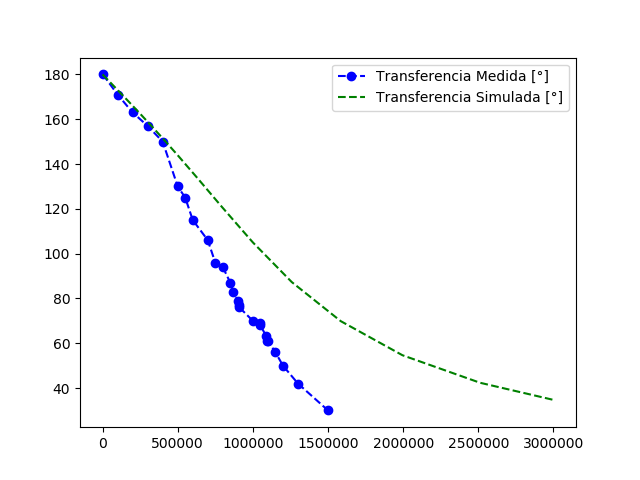
\includegraphics[width=0.8\textwidth]{Ejercicio1/Imagenes/BodephC3.png}
	\caption{Diagrama de Bode en fase Caso 3.}
	\label{fig:BodephC3}
\end{figure} 

Para las mediciones del tercer caso, se presentó el problema de que se dificultó la toma de mediciones, debido a que, se estaba atenuando la señal a medir, por lo tanto se encontraba cerca del piso de ruido a altas frecuencias. Algo que se puede apreciar en esta medición es la aparición de un sobrepico. Las mismas fueron hechas con una punta \textbf{x10}, la cual introdujo un polo adicional, generando un sistema de segundo orden, justificando la aparición de dicho sobrepico.

A continuación se presentan las mediciones realizadas para el circuito no inversor.

\begin{figure}[H]	
	\centering
	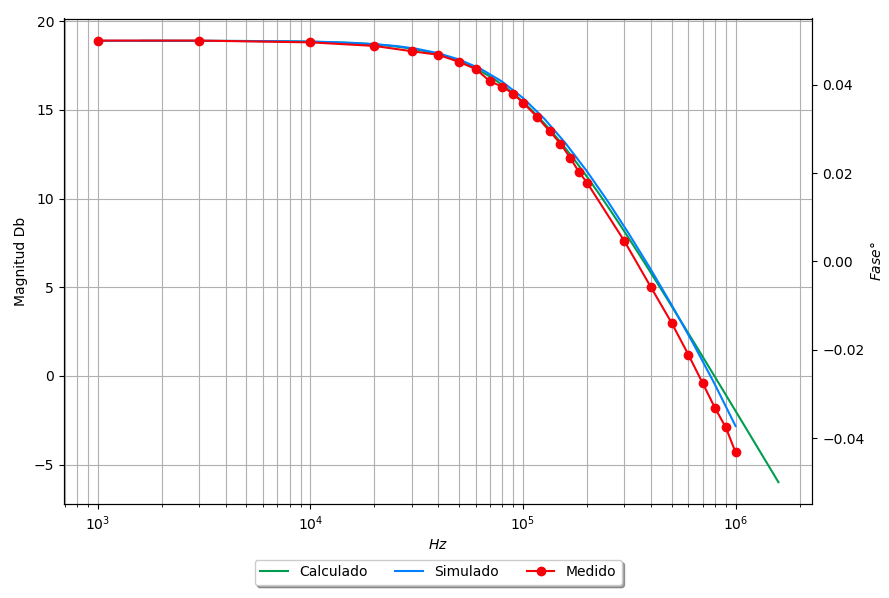
\includegraphics[width=0.8\textwidth, trim = {0 0 2cm 0},clip]{Ejercicio1/Imagenes/BodeC1_noinv.png}
	\caption{Diagrama de Bode en amplitud Caso 1.}
	\label{fig:BodeC1_noinv}
\end{figure} 
\begin{figure}[H]	
	\centering
	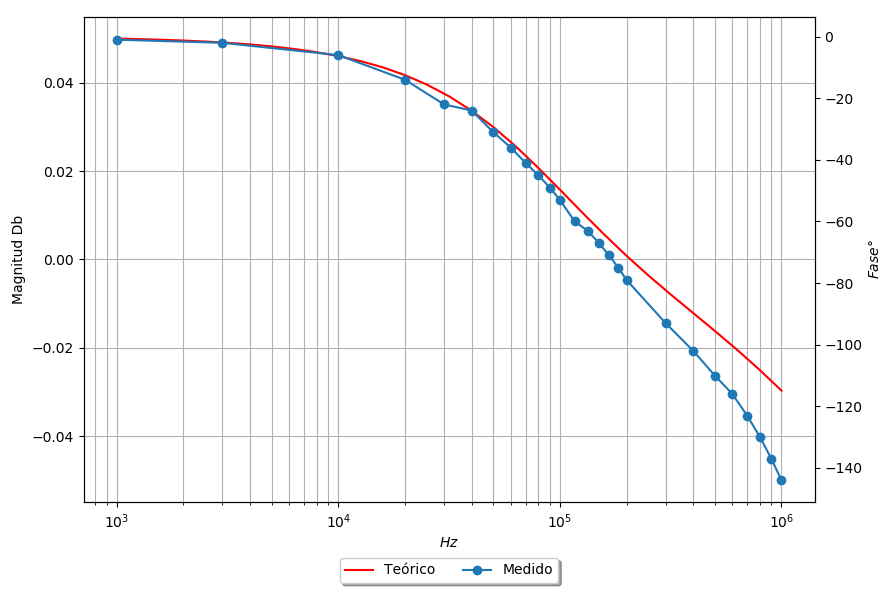
\includegraphics[width=0.8\textwidth, trim = {2.2cm 0 0 0},clip]{Ejercicio1/Imagenes/BodephC1_noinv.png}
	\caption{Diagrama de Bode en fase Caso 1.}
	\label{fig:BodephC1_noinv}
\end{figure} 

\begin{figure}[H]	
	\centering
	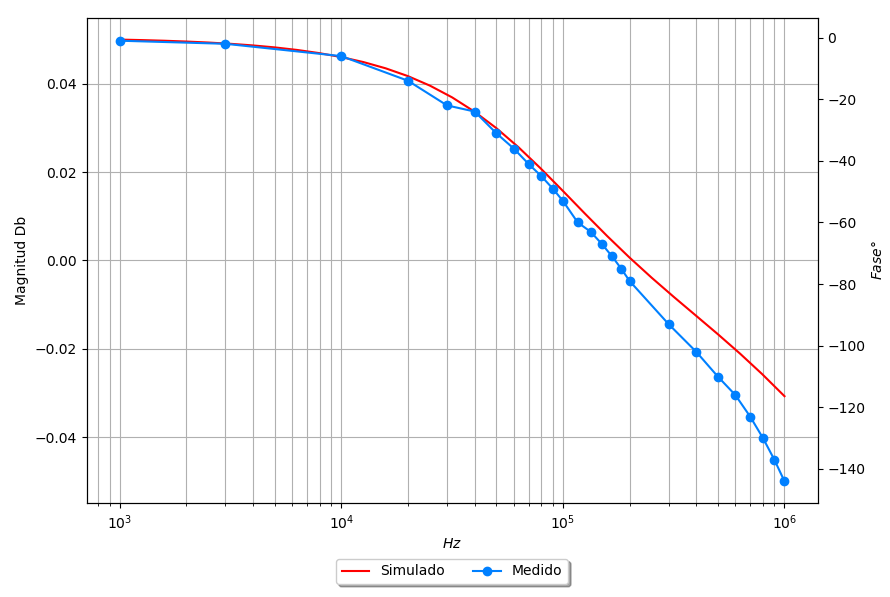
\includegraphics[width=0.8\textwidth, trim = {0 0 2cm 0},clip]{Ejercicio1/Imagenes/BodeC2_noinv.png}
	\caption{Diagrama de Bode en amplitud Caso 2.}
	\label{fig:BodeC2_noinv}
\end{figure} 
\begin{figure}[H]	
	\centering
	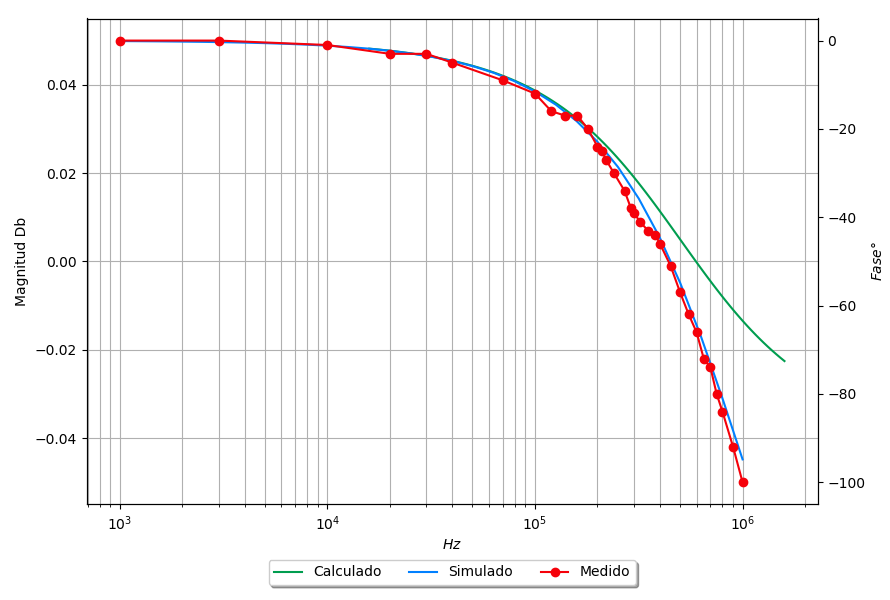
\includegraphics[width=0.8\textwidth, trim = {2.2cm 0 0 0},clip]{Ejercicio1/Imagenes/BodephC2_noinv.png}
	\caption{Diagrama de Bode en fase Caso 2.}
	\label{fig:BodephC2_noinv}
\end{figure} 

\begin{figure}[H]	
	\centering
	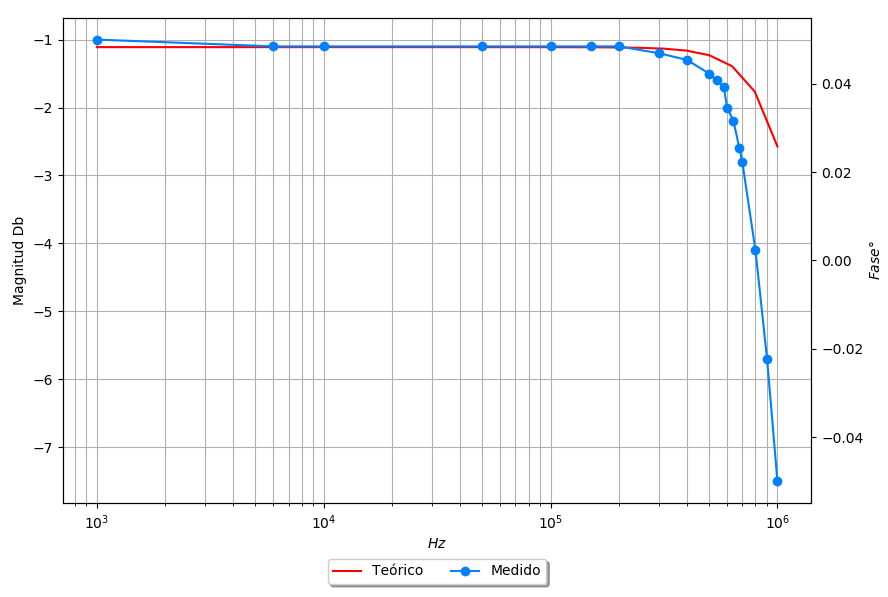
\includegraphics[width=0.8\textwidth, trim = {0 0 2cm 0},clip]{Ejercicio1/Imagenes/BodeC3_noinv.png}
	\caption{Diagrama de Bode en amplitud Caso 3.}
	\label{fig:BodeC3_noinv}
\end{figure} 
\begin{figure}[H]	
	\centering
	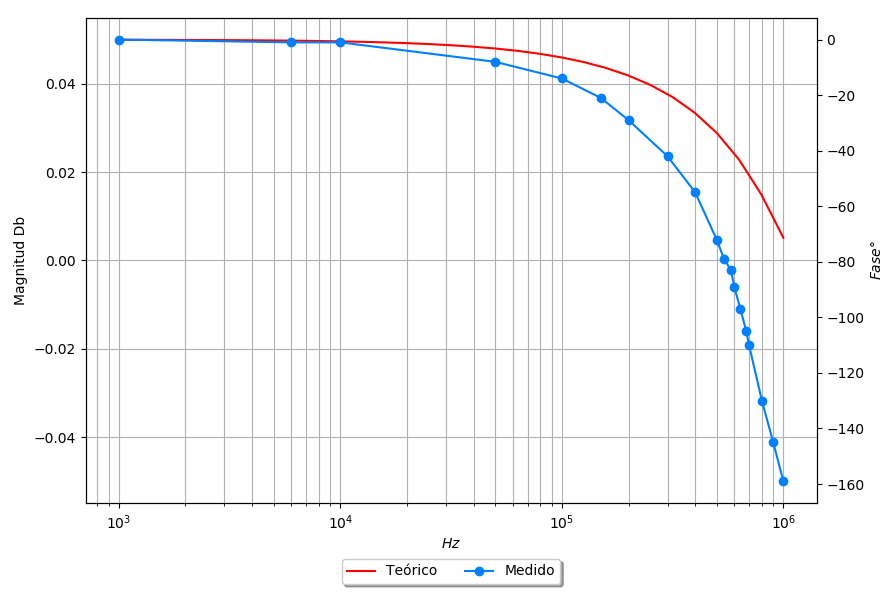
\includegraphics[width=0.8\textwidth, trim = {2.2cm 0 0 0},clip]{Ejercicio1/Imagenes/BodephC3_noinv.png}
	\caption{Diagrama de Bode en fase Caso 3.}
	\label{fig:BodephC3_noinv}
\end{figure} 

Se puede observar en todos los casos como la frecuencia de corte de las transferencias son próximas, mientras que las transferencias medidas y simuladas difieren de la teórica. Esto es más evidente al observar las discrepancias en (\ref{fig:BodephC1_noinv}), (\ref{fig:BodephC2_noinv}) y (\ref{fig:BodephC3_noinv}) a altas frecuencias. Esto se debe a las puntas del osciloscopio cuyas capacitancias son de aproximadamente $80 \ pF$. Al pasar a las altas frecuencias, este capacitor genera un filtro de segundo orden con el polo ya existente, atenuando la tensión de salida del circuito y generando en consecuencia que esta sea comparable con el ruido existente y dificultando las mediciones.

\subsubsection{Limitaciones.}
Algunas limitaciones con las cuales se lidiaron al utilizar este operacional fueron la intervención del Slew-Rate, el efecto de Cross-Over y la saturación del mismo.

En el caso de que se quiera trabajar con una señal cuadrada de $1 \ Vpp$, en un rango de frecuencias de $0.3 \ MHz \sim 2 \ MHz$, con un Duty Cycle entre 20\% y 80\%, no será posible, dado que se presentaran problemas de Slew-Rate. Por otro lado, se observarán problemas de Cross-Over cuando la media de la señal no supere los $0.7 \ V$.
Viendo que el operacional LM324 no funciona para dichas aplicaciones, se encontraron X amplificadores operacionales que pueden ser utilizados con una señal de las características mencionadas. Considerando que posean un valor medio de $0 \ V$ y un DT de 50\% los cuales son: TL084,

\begin{center}
\textcolor{red}{\textbf{BUSCAR OPERACIONALES.}}
\end{center}

\end{document}

\subsection{Caracterización de Amplificadores Operacionales}

	
\subsection{Introducción teórica}


El objetivo de esta sección es comparar el comportamiento de dos amplificadores operacionales diferentes, analizando sus características principales, contrastando sus respectivos modelos teóricos, simulaciones y mediciones.

En la siguiente tabla se presentan algunas características otorgadas por los fabricantes sobre ambos integrados que serán de importancia en el  análisis que sigue:

\begin{table}[H]
\hspace*{-2cm} 
\begin{tabular}{|c|c|c|c|c|c|c|}
\hline
Amplificador   & $A_{vol}$ (dB)   & GBP (MHz)   & Slew-Rate ($\frac{V}{\mu s}$)   & V offset (mV)  & I bias (nA)  & $r_d$ \\ %k\Omega \\ \hline
$LM833$ & $110$ & $10-15$ & $7$   & $0,3$  & $300$ & no especifica \\ \hline
$NE5534$ & $25-100$    & $10$  & $7.5$   & $0,5-4$  & $500-1500$ &  $100 \ k\Omega$
\\ \hline
\end{tabular}
\caption{Datos op-amps.}
\label{tabla:caracteristicas_amps}
\end{table}

El circuito a trabajar es la configuración no inversora dada en la Figura (\ref{fig:consigna}), en la cual $R_1 = 3 \ k\Omega$, $R_2 = 240 \ k\Omega$ y $R_3 = 220 \ k\Omega$. Se utilizó esta misma configuración para ambos integrados.  

\begin{figure}[H]
\begin{center}
\begin{circuitikz}
	\node [op amp](A1){};
	\draw (A1.-) to[short] ++(-1.5,0) to[R, l_=$R_1$] ++(-1.5,0) to[short] ++(-1,0) node[ground]{};
	\draw (A1.-) node[label=south:$V^-$]{};
	\draw (A1.+) node[label=south:$V^+$]{};
	\draw (A1.-) to[short] ++(0,1.5) to[R, l = $R_2$] ++(3,0) to[short] ++(0,-2);
	\draw (A1.+) to[short] ++(-1,0) to[R, l = $R_4$] ++(0,-1.5) node[ground]{};
	\draw (A1.out) to[short, -o] ++(1,0) node[ocirc,label=right:$V_{out}$]{};
	\draw (A1.+) to[short] ++(-1,0) to[R, l= $R_3$] ++(-2,0) to[short, -o] node[ocirc,label=left:$V_{in}$]{} ++(-1,0);
	\end{circuitikz}
	\caption{Configuración no inversora.}
	\label{fig:consigna}
\end{center}
\end{figure}

\subsubsection{Respuesta en frecuencia}

Un amplificador operacional puede describirse mediante diferentes modelos. Un análisis inicial fue hecho en la sección anterior, no obstante aquí se profundizará más al respecto. Un esquema de la configuración no inversora completa puede verse en la Figura (\ref{fig:esquema_no_inversor}). 

\begin{figure}[H]	
	\centering
	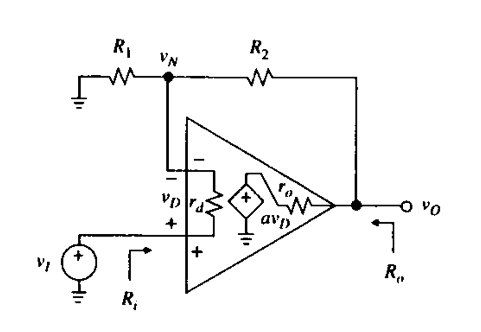
\includegraphics[width=\textwidth]{Ejercicio2/Imagenes/Rin_no_inversor.png}
	\caption{Esquema configuración no inversora completa.}
	\label{fig:esquema_no_inversor}
\end{figure}

Para el modelo ideal la resistencia $r_d$ es igual a infinito, mientras que $r_0$ es igual a cero y la ganancia es por ende, infinita. No obstante el caso analizado y medido dista mucho del ideal. En realidad se puede considerar a $A_0$ como un número muy grande, pero finito, al igual que $r_d$. En ese caso se considera que casi no circula corriente por $r_d$ y por ende la tension en el nodo N ($v_N$), es igual a $V_{in}$. La tension a la salida es a su vez:

\begin{equation}\label{eq:ganancia}
V_{out} = A_{vol}(v_D)
\end{equation}
con $v_D$ igual a la diferencia de tension entre el borne positivo y el negativo. 

Es posible también, realizar un divisor resistivo entre $R_2$ y $R_1$:

\begin{equation}
V_N = \frac{V_{out}R_1}{R_1 + R_2}
\end{equation}

Reemplazando en (\ref{eq:ganancia}):

\begin{equation}
V_{out} = A_{vol}(V_{in} - \frac{V_{out}R_1}{R_1 + R_2})
\end{equation}

Si resuelvo para $\frac{V_{out}}{V_{in}}$ y reordeno:

\begin{equation}\label{eq:transferencia_real}
\frac{V_{out}}{V_{in}} = \frac{A_{vol}}{1 + \frac{A_{vol}}{1 + \frac{R_2}{R_1}}}
\end{equation}

Cuando se realiza el límite de $A_vol$ tendiendo a infinito se llega a la expresión ideal:

\begin{equation}\label{eq:ganancia_ideal}
G_i = 1 + \frac{R_2}{R_1}
\end{equation}

El último modelo utilizado es el del polo dominante o compensación por frecuencia. Debido a que la mayoría de los amplificadores utilizan el feedback negativo como método para alcanzar altas ganancias, es posible que a altas frecuencias, imperfecciones dentro del chip generen que este feedback se de vuelta, causando que el amplificador oscile. 

%%Se puede incluir mñas teoría sobre compensación de polos

El modelo de polo dominante utilizado es el siguiente:

\begin{equation}\label{eq:polo_dominante}
A_{vol} = \frac{A_0}{1 + \frac{s}{\omega_p}}
\end{equation}

en el cual $\omega_p$ es del orden de los Hertz.
Si se reemplaza (\ref{eq:ganancia_ideal}) y (\ref{eq:polo_dominante}) en (\ref{eq:transferencia_real}), con un poco de trabajo matemático se llega a la siguiente fórmula normalizada:

\begin{equation}\label{eq:ganancia_completa_normalizada}
\frac{V_{out}}{V_{in}} = \frac{\frac{G_iA_0}{A_0 + G_i}}{1 + \frac{s}{\omega_p(1 + \frac{A_0}{G_i})}}
\end{equation}

Por último, un parámetro de vital importancia para el análisis de un amplificador operacional es su GBP, o el producto entre el ancho de banda del amplificador y la ganancia a la cual es medido. Para cualquier op-amp con polo dominante esta cantidad es una constante independiente de la ganancia a la cual es medida. El gain-bandwidth-product, es importante ya que, da una idea de la máxima ganancia que se puede extraer de un dispositivo a una frecuencia dada. El GBP para un amplificador operacional con polo dominante es igual a la siguiente expresión:

\begin{equation}\label{eq:GBP}
GBP = A_0\omega_p = G_{real}\omega_c
\end{equation}
con $\omega_c$ el polo del circuito completo.


\subsubsection{Impedancia de entrada}

Para analizar la impedancia de entrada teórica del circuito se utilizó el modelo completo con polo dominante del op-amp. Todo el análisis siguiente se hará a partir de la Figura (\ref{fig:esquema_no_inversor}), con la única diferencia de que se considerará además una resistencia en la entrada no inversora del circuito ($R_3$). La impedancia de entrada del circuito puede obtenerse poniendo una fuente de prueba $v$ a la entrada del circuito para luego usar la relación:

\begin{equation}\label{eq:zin}
Z_{in} = \frac{v}{i}
\end{equation}

En primer lugar se plantea la ecuación de corrientes en el nodo N:

\begin{equation}\label{eq:corrientes_N}
\frac{v - v_N}{R_3 + r_d} - \frac{v_N}{R_1} + \frac{A_{vol}v_D - v_N}{R_2} = 0
\end{equation}

Se por inspección que:

\begin{equation}\label{eq:v_N}
v - v_D = v_N = v - r_di
\end{equation}

Reemplazando (\ref{eq:v_N}) en (\ref{eq:corrientes_N}) y simplificando:

\begin{equation}
\frac{r_{di}}{R_3 + r_d} - \frac{v}{R_1} + \frac{r_{di}}{R_1} +\frac{A_{vol}r_{di} - v + r_{di}}{r_0 + R_2} = 0
\end{equation}

Si se factoriza la expresión anterior de un lado por i y del otro por v:

\begin{equation}
i \left(\frac{r_d}{r_d + R3} + \frac{r_d}{R_1} + \frac{A_{vol}r_d}{r_0 + R_2}\right) = v\left(\frac{1}{R_1} + \frac{1}{r_0 + R_2}\right)
\end{equation}

Si se reemplaza (\ref{eq:zin}) en la ecuación anterior se cancelan las corrientes. Luego resuelvo para $Z_i$ y después de reordenar la expresión resultante es la siguiente:

\begin{equation}\label{eq:zin_real}
Z_i = r_d \left(\frac{R_1 // (r_0 + R_2)}{r_d + R_3} + 1 + \frac{A_{vol}}{1 + \frac{r_0 + R_2}{R_1}} \right)
\end{equation}

Si se reemplaza $A_{vol}$ por su modelo de polo dominante y se reordena se llega a lo siguiente:

\begin{equation}\label{eq:zin_completa}
Z_i = r_d \left(1 + \frac{R_1 // (r_0 + R_2)}{r_d + R_3} + \frac{\frac{A_0}{1 + \frac{r_0 + R_2}{R_1}}}{1 + \frac{s}{\omega_p}}\right)
\end{equation}

Por último es importante mencionar el método de medición de $Z_i$. Para eso se modeló el circuito como si fuera un divisor resistivo, es decir, se colocó una resistencia extra de $1 \ k\Omega$ a la entrada del circuito y se midió cuanta tensión caía sobre dicha resistencia con el osciloscopio. Se hizo lo mismo para la fase, aunque los resultados finales pueden mejorarse. 


\subsection{Resultados experimentales LM833}

Con los valores de resistencias utilizados la ganancia ideal tiene un valor de 81, (\ref{eq:ganancia_ideal}), valor a tener en cuenta a la hora de medir, para evitar tener problemas con el slew rate o que el amplificador sature. Por lo anterior se utilizaron tensiones del orden de los milivoltios para medir la respuesta en frecuencia. De (\ref{eq:GBP}), considerando el peor caso para el GBP brindado por el fabricante $(10 \ Mhz)$, se obtiene que:

\begin{equation}\label{eq:frecuencia_corte_LM833}
f_c = \frac{GBP}{2\pi G_i} = 19649 \ Hz
\end{equation} 

Se toma $G_i$ ya que $A_0$ es considerablemente grande y por ende $G_i$ es cercano a $G_{real}$. 


Por último antes de pasar al análisis de la respuesta en frecuencia del circuito con el LM833, al realizarse las mediciones se observó que a medida que la frecuencia de la señal de entrada aumentaba aparecía un offset en la señal de salida. En otras palabras, había una componente de continua montada sobre la señal de salida, por ende el valor medio de la salida es diferente a $0 \ V$. A pesar de lo anterior, este fenómeno solo se pudo apreciar a frecuencias relativamente altas (orden de los Megahertz). Debido a que el LM833 tiene una impedancia entre sus bornes muy grande (orden de los Megaohm), a frecuencias bajas no se observa un offset en la salida. Pero a medida que la frecuencia aumenta, a su vez disminuye la impedancia de entrada del circuito y así, se hace comparable el valor de $R_3$ con el de $Z_i$. Lo anterior ocasiona que haya una corriente entrando al amplificador, llámese Input Bias Current, que haya una caída de tensión no deseada a la entrada y se degrade la condición de Tierra virtual. 

\subsubsection{Respuesta en frecuencia}

Ya habiendo descrito los modelos teóricos y su respectivo método de medición, se procede a presentar los gráficos obtenidos en los cuales se superpone el modelo teórico, las simulaciones realizadas en LTSpice y los datos medidos:

\begin{figure}[H]	
	\centering
	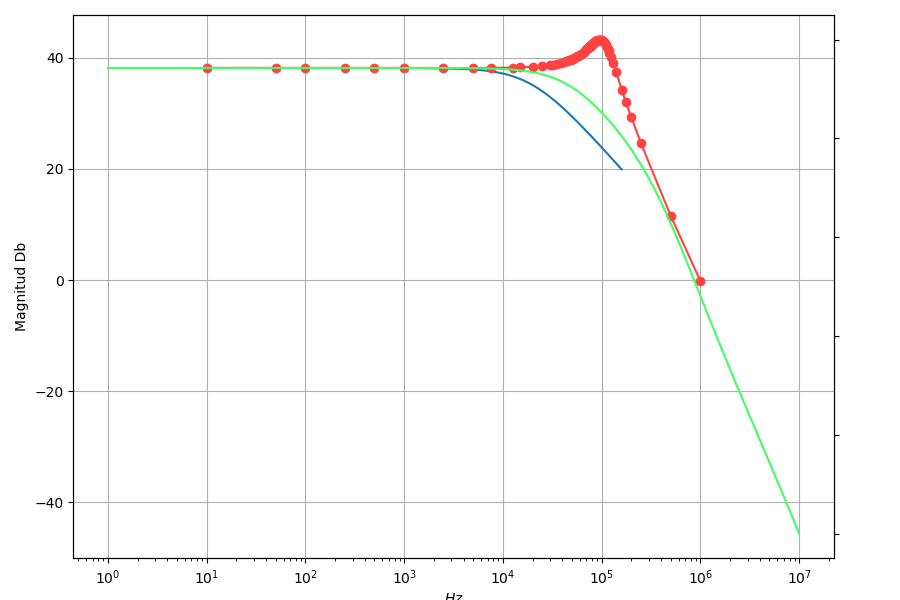
\includegraphics[width=\textwidth]{Ejercicio2/Imagenes/Bode_Amp_LM833.png}
	\caption{Diagram de Bode en amplitud para LM833.}
	\label{fig:bode_amp_LM833.}
\end{figure}

\begin{figure}[H]	
	\centering
	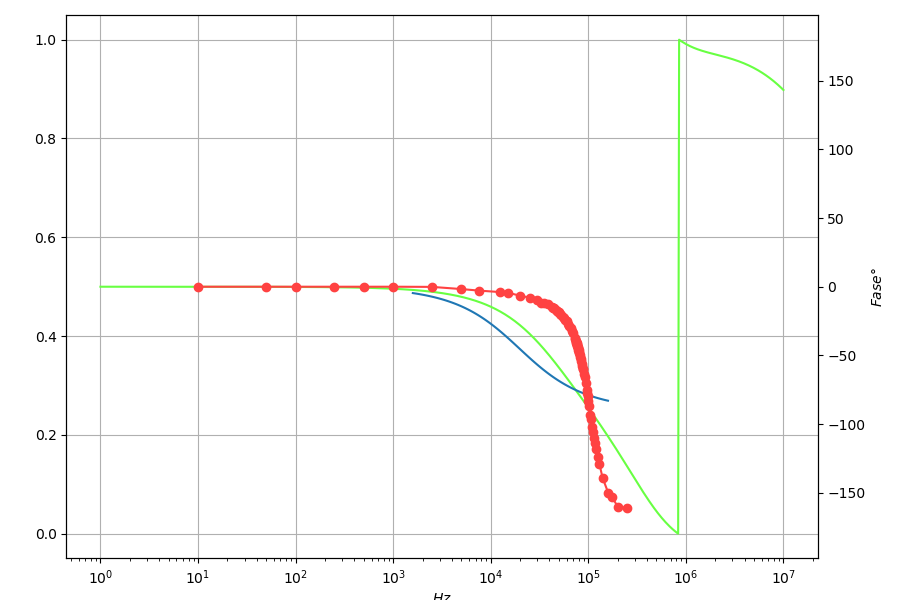
\includegraphics[width=\textwidth]{Ejercicio2/Imagenes/Bode_Fase_LM833.png}
	\caption{Diagram de Bode en fase para LM833.}
	\label{fig:bode_fase_LM833.}
\end{figure}

%%NO salieron colores, agregar despues


En primer lugar puede verse en el gráfico (\ref{fig:bode_amp_LM833}) que la frecuencia de corte obtenida en (\ref{eq:frecuencia_corte_LM833}) concuerda con el modelo simulado. Lo que no concuerda con el modelo simualdo y menos aún con el teórico es el sobrepico medido. El resultado esperado era un circuito que se asemeje a un pasa-bajos de primer orden, no obstante el sobrepico indica que el circuito real obedece a un modelo de segundo orden. Se pueden buscar razones para explicar este resultado. Por el solo acto de medir se esta agregando una capacitancia de $11 \ pF$ debido a las puntas, además se tiene que tener en cuenta la capacitancia de los terminales de los componentes y que el circuito fue medido en un protoboard, el cual agrega aproximadamente $2 \ pF$ por cada conexión hecha. El pico observado en un principio fue un problema para las mediciones, ya que el amplificador llegaba a su punto de saturación cerca del máximo. Más allá de esta anomalía el resto del gráfico es acorde a las simulaciones y la teoría. 

Por otro lado puede hacerse el mismo análisis con la fase del circuito. Teoricamente uno esperaría medir un circuito de primer orden, en el cual es desfase máximo es de 90 grados, pero las evidencias empíricas demuestran lo contrario, se esta trabajando con un circuito de segundo orden y un desfase de 180 grados. Incluso puede observarse a que a altas frecuencias hay un salto en la fase simulada, comportamiento que no logró medirse en el laboratorio.

Un primer paso para mejorar las mediciones es realizar el circuito en una PCB y asi disminuir las capacidades parásitas. Agregado a lo anterior, una solución al problema de las capacidades parásitas es incluir algún tipo de circuito de compensación, similar a lo que hacen los fabricantes al agregar un capacitor dentro del op-amp para evitar la inversión del feedback. El fabricante no incluyó ningún tipo de circuito de compensación recomendado en el caso del LM833 .

\subsubsection{Impedancia de entrada}

Para graficar la impedancia de entrada teórica hacen falta datos respecto de las resistencias internas del amplificador que no fueron dados por el fabricante. Por lo tanto se limita a presentar los gráficos correspondientes a las mediciones y las simulaciones:

\begin{figure}[H]	
	\centering
	\includegraphics[width=\textwidth]{Ejercicio2/Imagenes/Zin_A_LM833_Simulado.png}
	\caption{Impedancia de entrada LM833 en amplitud simulada.}
\end{figure}

\begin{figure}[H]	
	\centering
	\includegraphics[width=\textwidth]{Ejercicio2/Imagenes/Zin_F_LM833_Simulado.png}
	\caption{Impedancia de entrada LM833 en fase simulada.}
\end{figure}

\begin{figure}[H]	
	\centering
	\includegraphics[width=\textwidth]{Ejercicio2/Imagenes/Zin_A_LM833_Medido.png}
	\caption{Impedancia de entrada LM833 en amplitud medida.}
\end{figure}

\begin{figure}[H]	
	\centering
	\includegraphics[width=\textwidth]{Ejercicio2/Imagenes/Zin_F_LM833_Medido.png}
	\caption{Impedancia de entrada LM833 en fase medida.}
\end{figure}

Es importante destacar que a frecuencias menores a los $100 Hz$ fue imposible la medir una caída de tension en la resistencia colocada en serie delante del circuito. Es importante observar la expresión obtenida en \ref{eq:zin_completa} y ver como se comporta a medida que varía la frecuencia. A frecuencias bajas la resistencia tiende $r_d$, es decir un valor muy grande, razón por la cual fue imposible medir caídas de tensión. Luego lo esperado es que el modulo de la impedancia baje hasta llegar a un valor constante, comportamiento que se evidencia en los gráficos anteriores. En resumen, se puede observar una linea de tendencia en las mediciones que concuerdan con el modelo, para mejorar las mediciones una posibilidad es utilizar el analizador de impedancias en vez del osciloscopio.


\subsection{Resultados experimentales NE5534}

Debido a que el dato de GBP dado por el fabricante es el mismo que el valor mínimo para el amplificador anterior la frecuencia de corte del circuito teórica será aproximadamente la misma, considerando que se tiene la misma ganancia ideal. No obstante lo anterior, el NE5534 posee un $A_{vol}$ con muchísima disperisón, por lo que se tomó el valor típico del mismo. Además la resistencia de entrada en este caso es mucho menor, igual a $100k\Omega$ en el mejor de los casos. Debido a esto, cuando se comenzó a medir con $R_3 = 220k\Omega$ no se logró que el circuito funcionara. Como $R_3$ era del mismo orden, en este caso mayor, que $R_{in}$ el circuito funcionaba como un divisor resistivo que además amplificada el ruido que entraba al sistema. En la figura siguiente se ve el efecto medido en un principio:


\begin{figure}[H]	
	\centering
	\includegraphics[width=\textwidth, trim = {0 3.3cm 0 2cm},clip]{Ejercicio2/Imagenes/ruido.png}
	\caption{Ruido medido en NE5534.}
	\label{fig:ruido}
\end{figure}

Para evitar lo anterior, se reemplazó la resistencia $R_3$ por una igual a $22 \ k\Omega$. El segundo efecto visto fue el de un offset en la señal de salida. Para este operacional el offset sí podía apreciarse a bajas frecuencias y era muy notorio a medida que éstas aumentaban. Para evitar lo anterior el fabricante ofrece un circuito de compensación en su datasheet, en el cual se le agrega un capacitor adicional al circuito. A pesar de eso las mediciones fueron realizadas sin el circuito de compensación.

\subsubsection{Respuesta en frecuencia}
Los resultados obtenidos se presentan en los gráficos a continuación:

\begin{figure}[H]	
	\centering
	\includegraphics[width=\textwidth]{Ejercicio2/Imagenes/Bode_Amp_NE5534.png}
	\caption{Diagrama de Bode en amplitud para NE5534}
	\label{fig:bode_amp_NE5534}
\end{figure}

\begin{figure}[H]	
	\centering
	\includegraphics[width=\textwidth]{Ejercicio2/Imagenes/Bode_Fase_NE5534.png}
	\caption{Diagrama de Bode en fase para NE5534}
	\label{fig:bode_amp_NE5534}
\end{figure}

Al igual que en el amplificador anterior, se midió un sobrepico cercano a la frecuencia de corte del circuito. En este caso, dicho sobrepico es aún mayor que para el LM833, lo que indica mayores capacidades parásitas. Además la frecuencia a la que ocurre dicho sobrepico es mayor a la frecuencia teórica calculada anteriormente. Debido a que la ganancia ideal es igual para ambas configuraciones, la única diferencia está el GBP del integrado. Es fácil ver entonces que la ganancia en dBS para el NE5534 alcanza un sobrepico mayor que el LM833 pero es menor en el segmento en el que es constante. De esta manera queda demostrado el efecto del producto de ancho de banda en un operacional y como varía de modelo en modelo. En el NE5534 se logra un mayor ancho de banda, a cambio de perder un poco de ganancia, mientras que en el LM833 ocurre lo contrario. En ambos gráficos puede verse también que debido a las capacidades parásitas el circuito se comporta como uno de segundo orden experimentalmente.

Además de lo anteriormente descrito las mediciones concuerdan bastante bien con los modelos en las secciones en que son cuasi-lineales en el caos de la amplitud, y se puede observar una tendencia similar en el diagrama de fase, a pesar de haberse medido esencialmente un circuito de segundo orden.

\subsubsection{Impedancia de entrada}
El análisis de la impedancia de entrada para el NE5534 es idéntico al chip anterior, con la salvedad de que si pudieron medirse impedancias a menores frecuencias gracias a que la impedancia de entrada del circuito es muchísimo menor para este operacional. Para realizar estas mediciones tampoco se recurrió al circuito de compensación.


\begin{figure}[H]	
	\centering
	\includegraphics[width=\textwidth]{Ejercicio2/Imagenes/Zin_A_NE5534_Simulado.png}
	\caption{Impedancia de entrada NE5534 en amplitud simulada.}
\end{figure}

\begin{figure}[H]	
	\centering
	\includegraphics[width=\textwidth]{Ejercicio2/Imagenes/Zin_F_NE5534_Simulado.png}
	\caption{Impedancia de entrada NE5534 en fase simulada.}
\end{figure}

\begin{figure}[H]	
	\centering
	\includegraphics[width=\textwidth]{Ejercicio2/Imagenes/Zin_A_NE5534_Medido.png}
	\caption{Impedancia de entrada NE5534 en amplitud medida.}
\end{figure}

\begin{figure}[H]	
	\centering
	\includegraphics[width=\textwidth]{Ejercicio2/Imagenes/Zin_F_NE5534_Medido.png}
	\caption{Impedancia de entrada LM833 en fase medida.}
\end{figure}

Al igual que en el integrado anterior, se observa una tendencia que concuerda entre la simulación y las mediciones. A pesar de lo anterior, más mediciones con una mayor precisión son requeridas para sacar mejores conclusiones al respecto.
\subsection{Aplicaciones}
Los dos amplificadores aquí tratados poseen características que los hacen deseables para cierto tipo de aplicaciones. Ambos poseen un $A_{vol}$, y por consiguiente, una ganancia relativamente grande en un ancho de banda amplio. Lo anterior hace que ambos amplificadores sean útiles en aplicaciones de Audio y preamplificación, ya que el rango de frecuencias en el que se manejan concuerda con ese tipo de aplicaciones. Además, el LM833 posee una impedancia de entrada muy grande y una impedancia de salida muy chica, lo que lo convierte en un gran adaptador de impedancias, no así el otro op-amp analizado. Una desventaja del LM833 es que no hay una manera de integrar un circuito de balance al mismo, al contrario que con el NE5534. 


\subsection{Conclusiones}

En el diseño de un circuito hay que tener en cuenta diversos factores a la hora de elegir que elemento utilizar. En el caso de los amplificadores operacionales, no solo importa la ganancia sino que es de vital importancia analizar las impedancias de entrada y de salida. Como ocurrió en el desarrollo de este ejercicio, a la hora de medir dichos parámetros fueron fundamentales a la hora de armar los circuitos deseados. El caso analizado es quizás el más simple de los circuitos, no así el menos importante de comprender. En caso de tener circuitos con diversas fases el no tener en cuenta factores como los nombrados anteriormente puede significar la diferencia entre recibir una señal limpia o medir ruido a la salida de un sistema. Por eso, queda como conclusión final que es deber de cualquier diseñador tener en cuenta la mayor cantidad posible de variables en la implementación de un circuito.

\subsection{Medición de Bias}

	%\documentclass[a4paper]{article}
%\usepackage[spanish]{babel}
%\usepackage[utf8]{inputenc}
%\usepackage{float}
%\usepackage{graphicx}
%\usepackage[american voltage]{circuitikz}
%\usepackage{amsmath}
%\usepackage{xcolor}
%\usepackage{caption}
%\usepackage{subcaption}
%\usepackage[bottom]{footmisc}
\documentclass[a4paper]{article}
\usepackage[utf8]{inputenc}
\usepackage[spanish, es-tabla, es-noshorthands]{babel}
\usepackage[table,xcdraw]{xcolor}
\usepackage[a4paper, footnotesep = 1cm, width=20cm, top=2.5cm, height=25cm, textwidth=18cm, textheight=25cm]{geometry}
%\geometry{showframe}

\usepackage{tikz}
\usepackage{amsmath}
\usepackage{amsfonts}
\usepackage{amssymb}
\usepackage{float}
\usepackage{graphicx}
\usepackage{caption}
\usepackage{subcaption}
\usepackage{multicol}
\usepackage{multirow}
\setlength{\doublerulesep}{\arrayrulewidth}
\usepackage{booktabs}

\usepackage{hyperref}
\hypersetup{
    colorlinks=true,
    linkcolor=blue,
    filecolor=magenta,      
    urlcolor=blue,
    citecolor=blue,    
}

\newcommand{\quotes}[1]{``#1''}
\usepackage{array}
\newcolumntype{C}[1]{>{\centering\let\newline\\\arraybackslash\hspace{0pt}}m{#1}}
\usepackage[american]{circuitikz}
\usetikzlibrary{calc}
\usepackage{fancyhdr}
\usepackage{units} 

\graphicspath{{../Ejercicio-1/}{../Ejercicio-2/}{../Ejercicio-3/}{../Ejercicio-4/}}

\pagestyle{fancy}
\fancyhf{}
\lhead{22.01 Teoría de Circuitos}
\rhead{Mechoulam, Lambertucci, Rodriguez Turco, Londero, Galdeman}
\rfoot{\centering \thepage}

	\subsection{Introducción}
	Los amplificadores de instrumentación, también conocidos como \textbf{IN-AMP},  son utilizados para amplificar con alta precisión las señales provenientes de diversas unidades de adquisición de datos que no poseen la amplitud suficiente o estan demasiado contaminadas por ruido externo como para poder ser aprovechadas.
	\subsubsection{Diferencias entre \textbf{IN-AMP} y \textbf{OP AMP}}
	A simple vista un \textbf{IN-AMP} puede ser fácilmente confundido con un \textbf{OP AMP} dado que tiene varios rasgos en común. En primer lugar ambos dispositivos amplifican una señal diferencial, es decir que multiplican por un cierto factor la diferencia de potencial entre sus terminales de entrada. Por otro lado también poseen una elevada impedancia de entrada (del orden de los Megaohms) y una muy baja impedancia de salida de unos pocos ohms.
	No obstante, podemos notar algunas diferencias fundamentales entre ambos. Por ejemplo, para configurar la ganancia a lazo cerrado de un amplificador operacional se debe ajustar mediante resistores de retro-alimentación externos mientras que en un amplificador de instrumentación la ganancia puede venir predefinida por el fabricante o ajustada mediante una única \textbf{resistencia externa} denominada usualmente como \textbf{$R_{gain}$}.
	En caso de que se desee amplificar una señal diferencial el amplificador de instrumentación eliminara cualquier componente de señal común a ambas entradas como puede ser un offset de continua o simplemente ruido. Esta característica es la que hace especiales a los amplificadores de instrumentación ya que permiten reducir de manera significativa el ruido de las señales recibidas.  
	Por el contrario, los amplificadores operacionales tradicionales que no están diseñados para eliminar este tipo señales no deseadas.

	
	\subsection{Características del IN-AMP}
	El circuito a analizar es una variante de los famosos amplificadores de instrumentación que utilizan 3 amplificadores operacionales que se puede observar en la figura debajo.
	%Imagen del amplificador de instrumentación con 3 op-amps
	\begin{figure}[H]
		\centering		
		\includegraphics[width=\linewidth]{./ImagenesVarias/inAmp3Opamp}
		%TODO revisar footnote imagen 
		\caption{Clásico amplificador de instrumentación con 3 Opamps}
	\end{figure}
	%\footnote{Imagen extraída de: \textit{A designer's guide to Sinstrumentation amplifiers}
		
	Como se puede apreciar a la izquierda de la línea punteada se han colocado un par de buffers con ganancia. El objetivo de los mismos es de el de aumentar significativamente la impedancia de entrada del in-amp para independizarla lo más posible de la impedancias de las fuentes ya que este pueden ser muy altas o estar desbalanceadas. También ofrece la ventaja de no cargar a la fuente, lo cual es de gran relevancia al trabajar con señales pequeñas. Además le otorga una cierta ganancia a la señal de entrada. Este aspecto del circuito se debe tener en cuenta para evitar la saturación de los op-amps y perder la efectividad del circuito. Analizaremos esta y otras situaciones en secciones posteriores.
	En nuestro caso se trabajara con la versión de 4 amplificadores operacionales.
	
	\begin{figure}[H]
		\centering
		\includegraphics[width=\linewidth]{./ImagenesVarias/inAmpSch.png}
		\caption{Amplificador de instrumentación de 4 op-amps}
	\end{figure}

	Haciendo uso de la herramienta de análisis simbólico \textit{SapWin \footnote{SapWin es una programa de análisis y simulación de circuitos desarrollado por la \textit{Universitá degli studi Firenze}}} obtenemos la siguiente expresión para la ganancia ideal de amplificador de instrumentación:
	\begin{equation}
			V_{out}=\frac{-V_1 R_2 R_4 R_7 - 
			V_1 R_2 R_3 R_7 +
			V_2 R_2 R_3 R_7+
			V_2 R_2 R_3 R_6
		}{R_1 R_4 R_7}
		\label{eqn:idealTrans}
	\end{equation}

	
	Notamos que en la situación ideal tanto las resistencias $R_5$ y $R_9$ no afectan la ganancia del circuito.
	\subsubsection{Relaciones entre los componentes}
	Una de las finalidades del amplificador de instrumentación es la de eliminar aquellas señales que sean comunes a las señales de entrada.
	Por tal motivo comenzaremos por establecer condiciones que nos permitan eliminarlas. 
	Para eso aplicaremos superposición y analizaremos los efectos de $V_{CM}$ sobre la relación anterior.
	
	\begin{figure}[H]
		\centering
		\includegraphics[width=\linewidth]{./ImagenesVarias/inAmpVCM.png}
		\caption{Amplificador de instrumentación de 4 op-amps en modo común}
	\end{figure}
	Obteniendo como transferencia:
	\begin{equation}
		\frac{V_{out}}{V_{CM}}=
		\frac{-R_2 R_4 R_7 - 
			R_2 R_3 R_7 +
			R_2 R_3 R_7+
			R_2 R_3 R_6
		}{R_1 R_4 R_7}
	\end{equation}
		
	Como se quiere que aquellas señales comunes a ambas entrada sean eliminadas pedimos $V_{out}=0$.
	Entonces obtenemos:
		\begin{equation}
		 0=\frac{-V_{CM} R_2 R_4 R_7 - 
				V_{CM} R_2 R_3 R_7 +
				V_{CM} R_2 R_3 R_7+
				V_{CM} R_2 R_3 R_6
			}{R_1 R_4 R_7} 
		\end{equation}
	
	Simplificando
	\begin{equation}
		R_7(R_4+R_3)=R3(R7+R6)
	\end{equation}
	
	\begin{equation}
		R_7R_4+ R_3R_7=R_3R_7+R_3R_6
	\end{equation}
	Cancelando los términos comunes a ambos miembros
	\begin{equation}
		R_7R_4=R_3R_6
	\end{equation}
	Por lo tanto llegamos a:
	\begin{equation}
		\frac{R_4}{R_6}=\frac{R_3}{R_7}  %Relación entre las resistencias de la etapa de amplificación
	\end{equation}

	Aplicando estas relaciones a \eqref{eqn:idealTrans} obtenemos:
	\begin{equation}
		V_{out} = (V_2-V_1)\left[\frac{R_2}{R_1}(1+\frac{R_3}{R_4})\right]
	\end{equation}
En nuestro afán de conseguir una amplificación de 137,32 se realizaron las siguientes consideraciones en busca de conseguir la configuración más simétrica posible.
En primer lugar dadas las limitaciones de las tolerancias de los componentes se decidió implementar un amplificador de instrumentación con una ganancia de 137,5 veces. Sí bien se podría haber intentado calibrar la ganancia del mismo mediante el uso de resistores variables, debemos tener en cuenta que los presets no son ajustables con la suficiente precisión y estos además cuentan con su correspondiente tolerancia. Por otro lado a causa de vibraciones o movimientos bruscos los mismos podrían cambiar su valor forzando al usuario a chequear sus valores previo al uso. 
En segundo lugar se eligieron que las resistencias $R_3$ y  $R_4$ tomasen el mismo valor. Este decisión obligara a que $R_7$ y  $R_6$ también sean iguales. Por lo tanto conseguimos mucha simetría en la primera etapa

\begin{equation}
	V_{out} = (V_2-V_1)\left[2 \frac{R_2}{R_1}\right]
\end{equation}

Luego se eligió $R_2$ del mismo orden de magnitud que $R_1$ de forma tal que el factor de \textbf{2} que apareció previamente sea cancelado y $R_2$ controle por completo la ganancia. Esta $R_2$ fue armada mediante 2 resistores SMD en serie.

\begin{table}[H]
	\centering
	\begin{tabular}{lll}
		Componente  & Valor        	   & Tolerancia \\
		\\
		$R_1$       & 2K$\Omega$   	   & 1\%        \\
		$R_2$       & 130K$\Omega$ 	   & 1\%        \\
		$R_{2'}$  	& 7,5K$\Omega$     & 1\%        \\
		$R_3$ 		& 10K$\Omega$      & 1\%		\\
		$R_4$		& 10K$\Omega$      & 1\%        \\
	    $R_5$		& 10K$\Omega$      & 1\%        \\
	    $R_6$		& 10K$\Omega$      & 1\%        \\
	    $R_7$		& 10K$\Omega$      & 1\%        \\
	    $R_8$		& 2K$\Omega$       & 1\%        \\
 	    $R_9$		& 130K$\Omega$     & 1\%        \\   
		$R_{9'}$	& 7,5K$\Omega$     & 1\%        \\
			\end{tabular}
		\caption{Tabla de valores de componentes del IN-AMP al 1\%}
\end{table}

\begin{figure}[H]
	\centering
	\includegraphics[width=\linewidth]{./ImagenesVarias/IN-AMP-CON-VALORES.png}
	\caption{IN-AMP con los valores elegidos}
\end{figure}

  Cabe destacar que el orden de magnitud de los componentes se baso en que los amplificadores de instrumentación comerciales son fabricados con resistencias en el orden de los K-ohms.
  
  Como fue antes mencionado, el amplificador de instrumentación debe poseer, idealmente, impedancia de entrada infinita. Para poder aproximarnos lo más posible a este ideal se decidió utilizar el amplificador operacional \textbf{TL084} que posee una impedancia de entrada de 1 Tera-Ohm ($10^{12}\Omega$). Otra ventaja de elegir este operacional es que se consiguen en un solo integrado que contiene a los de 4 op-amps dentro de un mismo integrado lo cual disminuye las variaciones por cambios de temperatura dado que se encuentran los 4 bajo las mismas condiciones de operación.
  
\subsection{Efecto de las tolerancias}
Cuando se plantearon los primeros amplificadores diferenciales se utilizaron configuraciones simples como la exhibida debajo, ya se conocía que los resistores $R_1$, $R_2$, $R_3$ y $R_4$ debían estar apropiadamente balanceados con el fin de maximizar el rechazo en modo común. 
\begin{figure}[H]
	\centering
	\includegraphics[width=\linewidth]{./ImagenesVarias/AmplificadorDiferencial.PNG}
	\caption{Amplificador diferencial}
\end{figure}  

Sin embargo las tolerancias de los componentes no lo permiten. Es por tal motivo que para alcanzar dicha precisión los fabricantes construyen dichas resistencias, mediante técnicas láser durante el proceso de fabricación del IC con el fin de minimizar esas diferencias.

El modelo más sofisticado y robusto que se implemento presenta mejoras muy notables por sobre su antecesor. No obstante, estas mejoras también traen nuevos desafíos dado que se añaden más componentes resistivos al sistema.

Usando resistencias al 1\% obtenemos la siguiente simulación de Montecarlo para en modo diferencial

\begin{figure}[H]
	\centering
	\includegraphics[width=\textwidth]{./ImagenesDeSimulaciones/MonteCarloModoDiferencialGrande.png}
	\caption{Montecarlo en modo diferencial}
\end{figure}  
Como podemos notar, las tolerancias no afectan significativamente su desempeño en modo diferencial.

Sin embargo podemos realizar más observaciones en cuanto a su desempeño en modo comúm
\begin{figure}[H]
	\centering
	\includegraphics[height=0.3\textheight]{./ImagenesDeSimulaciones/MonteCarloModoComunGrande1V.png}
	\caption{Montecarlo en modo común con 1 Vpp de entrada}
\end{figure} 
Este gráfico de bode pone en evidencia la importancia de que las resistencias poseean la mayor precisión posible.

Si la tensión en modo común se reduce vemos como mejora el rechazo en modo común.
\begin{figure}[H]
	\centering
	\includegraphics[height=0.3\textheight]{./ImagenesDeSimulaciones/MonteCarloModoComunGrande100mv.png}
	\caption{Montecarlo en modo común con 100 mv de entrada}
\end{figure} 

También se intento ver los alcances de rechazo común frente a una continua
\begin{figure}[H]
	\centering
	\includegraphics[height=0.3\textheight]{./ImagenesDeOsciloscopio/ModoComunContinua.png}
	\caption{Rampa de 0 a 20V}
\end{figure} 

Vemos como el circuito es capaz de soportar hasta unos 5V de continua (como indica el cursor) antes de salir de su zona de operación.

\subsection{Respuesta en frecuencia}
Los amplificadores de instrumentación obtienen su mejor rendimiento en la rango de las frecuencias medias a bajas. Esta configuración exhibe un comportamiento del tipo pasabajos lo que provoca que no se obtenga la ganancia esperada a frecuencias elevadas.
\begin{figure}[H]
	\centering
	\includegraphics[height=0.3\textheight]{./ImagenesVarias/BODE_MAG.PNG}
	\caption{Bode de Magnitud}
\end{figure}


  
  
  
  
  
  
  
  
  
  
  
  
  
  
  
  
  
\subsection{Generación de señales con puente de Wheatstone}
Se diseño un puente de WheatStone para la generación de señales compuestas.
\begin{figure}[H]
	\centering
	\includegraphics[height=0.25\textheight]{./ImagenesVarias/wheatstone.png}
	\caption{Puente de WheatStone}
\end{figure}

Este método emula a un sensor que utilice un sistema tipo puente con un resistor variable que puede llegar a cambiar de valor según la temperatura, presión u alguna otra que ocasiona que su valor cambie.

\begin{figure}[H]
	\centering
	\includegraphics[height=0.3\textheight]{./ImagenesVarias/wheatstoneInAmp.png}
	\caption{IN-AMP con puente de WheatStone Acoplado}
\end{figure}

La tensión suministrada en la parte superior del puente permite que las variaciones de resistencia se traduzcan en una señal eléctrica.
Sin embargo es necesario poseer una cierta referencia para poder determinar si de hecho ocurrió un cambio. Es por es que el amplificador de instrumentación se vale del puente y de sus 2 bornes de salida para llevar acabo esta detección. La rama del puente que cuenta con sus resistores fijos proporcionara la tensión de referencia.
A la entrada del amplificador de instrumentación se le proporcionaran 2 señales. En primer tendremos la señal de referencia y por el otro la señal portadora de la perturbación.
Debemos notar que dado el diseño del amplificador de instrumentación de no haber diferencias entre las dos señales entonces en el caso ideal se debería observar una salida nula. 

Para el armado del puente se eligieron resistores con tolerancias del 1\% para mantener el puente lo más balanceado posible y maximizar el rechazo en modo común.
\begin{table}[H]
	\centering
	\begin{tabular}{lll}
		Componente  		& Valor        	& Tolerancia \\
		\\
		$R_1$       		& 10K$\Omega$   & 1\%        \\
		$R_2$       		& 10K$\Omega$ 	& 1\%        \\
		$R_{2'}$ Preset      & 1K$\Omega$ 	& 10\%        \\
		$R_3$  				& 10K$\Omega$   & 1\%        \\
		$R_4$ 				& 10K$\Omega$   & 1\%		\\
	\end{tabular}
	\caption{Tabla de valores de componentes del puente de WheatStone al 1\%}
\end{table}

El preset nos permite generar de manera artificial "la perturbación" sobre la señal.

\begin{figure}[H]
	\centering
	\includegraphics[height=0.3\textheight]{./ImagenesDeOsciloscopio/WheatStone1tierra1c1R.png}
	\caption{Amplificación de diferencias con puente de WheatStone}
\end{figure}
Notese la escala de las señales.
\subsubsection{Análisis de Tolerancias en el puente de WheatStone}


\subsubsection{Señales con y sin referencia a tierra}
La problemática al medir señales con entrada flotante, como pueden ser por ejemplo los transformadores o cualquier otro señal que se encuentre aislada de tierra radica en el hecho que las corrientes de bias del amplificador de instrumentación, no tanto las inherentes al dispositivo por cuestiones de fabricación, sino más bien aquellas desarrolladas por el aumento de la temperatura. Es de mayor relevancia en los \textbf{IN-AMP} desarrollados con transistores \textbf{FET} que, aunque tiene menores corrientes de bias a temperatura ambiente, estas se duplican cada 11 grados centigrados. Estas corrientes provocan que el amplificador de instrumentación conmute más rápidamente observándose cierto "ruido" en la señal de salida. Se recomienda siempre colocar un camino entre la fuente flotante y ground. Esto se puede lograr utilizando un resistor de entre $1M\Omega$ y  $10\Omega$

\begin{figure}[H]
	\centering
	\includegraphics[height=0.3\textheight]{./ImagenesDeOsciloscopio/WheatStoneTierra1.png}
	\caption{Amplificación de diferencias con puente de WheatStone con conexión a ground}
\end{figure}

\begin{figure}[H]
	\centering
	\includegraphics[height=0.3\textheight]{./ImagenesDeOsciloscopio/WheatstoneAislado.png}
	\caption{Amplificación de diferencias con puente de WheatStone con conexión a ground}
\end{figure}




 	
\begin{thebibliography}{9}
	
	\bibitem{Franco} 
	SERGIO, F. (2002). Design with operational amplifiers and analog integrated circuits. New York [etc.]: McGraw-Hill, pp.73-91.	
	
	\bibitem{Coughlin} 
	R. Coughlin and F. Driscoll, Circuitos integrados lineales y amplificadores operacionales. México: Prentice-Hall Hispanoamericana, 1998.
	
	\bibitem{dguideinamp}
	C. Kitchin and L. Counts, A designer's guide to instrumentation amplifiers. Norwood, Mass.: Analog Devices, 2006.
	
	\bibitem{an244}
	Jeffrey R. Riskin, A User's guide to IC instrumentation amplifiers. Norwood, Mass.: Analog Devices.
	
\end{thebibliography}


\subsection{Circuitos Integradores y Derivadores}

	\documentclass[a4paper]{article}
\usepackage[spanish]{babel}
%Para uso de palabras acentuadas
\usepackage[utf8]{inputenc}

\documentclass[a4paper]{article}
\usepackage[utf8]{inputenc}
\usepackage[spanish, es-tabla, es-noshorthands]{babel}
\usepackage[table,xcdraw]{xcolor}
\usepackage[a4paper, footnotesep = 1cm, width=20cm, top=2.5cm, height=25cm, textwidth=18cm, textheight=25cm]{geometry}
%\geometry{showframe}

\usepackage{tikz}
\usepackage{amsmath}
\usepackage{amsfonts}
\usepackage{amssymb}
\usepackage{float}
\usepackage{graphicx}
\usepackage{caption}
\usepackage{subcaption}
\usepackage{multicol}
\usepackage{multirow}
\setlength{\doublerulesep}{\arrayrulewidth}
\usepackage{booktabs}

\usepackage{hyperref}
\hypersetup{
    colorlinks=true,
    linkcolor=blue,
    filecolor=magenta,      
    urlcolor=blue,
    citecolor=blue,    
}

\newcommand{\quotes}[1]{``#1''}
\usepackage{array}
\newcolumntype{C}[1]{>{\centering\let\newline\\\arraybackslash\hspace{0pt}}m{#1}}
\usepackage[american]{circuitikz}
\usetikzlibrary{calc}
\usepackage{fancyhdr}
\usepackage{units} 

\graphicspath{{../Ejercicio-1/}{../Ejercicio-2/}{../Ejercicio-3/}{../Ejercicio-4/}}

\pagestyle{fancy}
\fancyhf{}
\lhead{22.01 Teoría de Circuitos}
\rhead{Mechoulam, Lambertucci, Rodriguez Turco, Londero, Galdeman}
\rfoot{\centering \thepage}

\usepackage{float}
\usepackage{graphicx}

\usepackage[american voltage]{circuitikz}

\usepackage{amsmath}

\usepackage{xcolor}

\usepackage{caption}
\usepackage{subcaption}

\begin{document}

\section{Circuitos integradores y derivadores}
\subsection{Introducción}
Los circuitos implementados con amplificadores operacionales permiten la implementación de diferentes configuraciones que resuelven problemas matemáticos. Con el diseño adecuado pueden usarse para resolver sistemas de ecuaciones diferenciales.
En este caso estudiaremos 2 bloques fundamentales. El circuito integrador y el derivador. Se analizaran sus características más relevantes así como también sus límites de uso y como extenderlos para aprovecharlos al máximo.

\begin{figure}[hbt!]
	\includegraphics[scale=1]{Ejercicio4/integrador.png}
	\caption{Circuito integrador} 
	
	\includegraphics{Ejercicio4/derivador}
	\caption{Circuito Derivador} 
	
\end{figure}

\subsection{Análisis previo del \textbf{LM833N}}
El amplificador a utilizar es el \textbf{LM833N} de STMicroelectronics. El mismo es un operacional de bajo ruido diseñado para aplicaciones relacionadas al manejo de audio.
En su hoja de datos podemos ver que posee un alto nivel Slew Rate de hasta 7 $\frac{V}{s}$, un GBP de 15MHz y una ganancia de tensión 
a lazo abierto típica de unos 110 dB. Notemos que también se indica que la ganancia mínima es de unos 90 dB. 


 \subsubsection{Cálculo de $A_{vol}$}
Para poder realizar los cálculos de transferencia y establecer sus correspondientes transferencias de teóricas primero debemos conocer $A_{vol}$ medido en veces. Para esto basta con tomar el valor de ganancia de tensión típica a veces.
$$A_{vol} = 10^{\frac{110}{20}}$$
$$A_{vol} \approx 316.227,77$$

\subsubsection{Cálculo de  la $f_p$, polo dominante}

Dado el \textbf{GBP} de 15MHz podemos fácilmente calcular la frecuencia de corte a lazo abierto

$$ f_p = \frac{15MHz}{A_{vol}} $$
$$ f_p \approx 47.44Hz$$

\section{Ganancia bajo diferentes condiciones de $A_{vol}$}
En esta sección analizaremos las características de la ganancia de tensión brindad por ambos circuitos bajo diferentes condiciones.

\subsection{$A_{vol}$ infinito}
En un circuito con amplificadores operacionales es deseable utilizar dispositivos con $A_{vol}$(ganancia a lazo abierto) lo más alto posible para que los modelos teóricos se aproximen a su implementación física.

Ambos circuitos adoptan la configuración de un circuito inversor y sus transferencias pueden ser descritas mediante
$$H(s)_{inv} = \frac{-\frac{Z_{Feed}}{Z_{in}}}
{1+\frac{1+\frac{Z_{Feed}}{Z_{in}}}{A_{vol}}} $$
La cual representa la función transferencia de un amplificador operacional no ideal.
Si consideramos $A_{vol}$ infinito obtenemos la transferencia para el inversor ideal:
$$H(s)_{inv} = \frac{-\frac{Z_{Feed}}{Z_{in}}}
				{1+\underbrace{\frac{1+\frac{Z_{Feed}}{Z_{in}}}{A_{vol}}}_{\text{\shortstack{$A_{vol}\rightarrow \infty$ \\ $\rightarrow 0$}}}}$$

$$H(s)_{ideal} =  -\frac{Z_{Feed}}{Z_{in}}$$

Entonces para el circuito integrador obtenemos:
$$H(s)_{\int_{}{}} = \frac{-1}{sCR} $$

Podemos corroborar que la acción de este circuito es integrar la señal de entrada al realizar la transformada inversa de Laplace
$$v_{out}(t) = \mathcal{L}^{-1}[X(s)H(s)_{\int_{}{}}]$$
$$v_{out}(t) = \mathcal{L}^{-1}[X(s)\cdot \frac{-1}{sCR}]$$
$$v_{out}(t)= \frac{-1}{CR} \cdot \int_{0}^{t}v_t dt$$            
\\
Por otro lado tenemos el circuito derivador:
$$H(s)_{\frac{d}{dt}}=-sCR$$
Análogamente aplicamos la anti-transformada de Laplace:

$$v_{out}(t) = \mathcal{L}^{-1}[X(s)H(s)_{\frac{d}{dt}}]$$

$$v_{out}(t) = \mathcal{L}^{-1}[X(s)\cdot (-sCR)]$$

$$v_{out}(t)= -CR \frac{d}{dt}v_t(t)$$       

Si bien, estos circuitos tienen la capacidad de realizar las operaciones antes mencionadas, en los párrafos siguientes estudiaremos su comportamiento y bajo que condiciones funcionan.

\subsubsection{Diagramas de Bode con $A_{vol}$ ideal}
\begin{figure}[H]
	\centering
	\includegraphics[width=\textwidth]{Ejercicio4/BODE-IDEAL-MAGNITUD-INTEGRADOR.png}
	\caption{Ganancia Ideal Circuito Integrador}
\end{figure}

Observamos que el integrador ideal tiene una muy alta ganancia a bajas frecuencias y muy baja cuando se acerca a los $10KHz$ lo cual limita su rango de operación.

\begin{figure}[H]
	\centering
	\includegraphics[width=\textwidth]{Ejercicio4/BODE-IDEAL-MAGNITUD-DERIVADOR.png}
	\caption{Ganancia Ideal Circuito Derivador}
\end{figure}
De modo contrario el derivador exhibe sus capacidades a altas frecuencias
\\*
En cuanto a la fase en ambos casos podemos observar como ver cómo las operaciones de integración y diferenciación introducen un desfase de $\pm90^{\circ}$ de la señal original según el caso. 
\begin{figure}[H]
	\centering
	\includegraphics[width=\textwidth]{Ejercicio4/BODE-IDEAL-FASE-INTEGRADOR.png}
	\caption{Fase Ideal Circuito Integrador}
\end{figure}

\begin{figure}[H]
	\includegraphics[width=\textwidth]{Ejercicio4/BODE-IDEAL-FASE-DERIVADOR.png}
	\caption{Fase Ideal Circuito Derivador}
\end{figure}

\subsection{$A_{vol}$ finito}
La ganancia a lazo abierto nunca es infinita en los amplificadores operacionales aunque por cuestiones de simplicidad podemos tratarlo como así fuese. En la introducción calculamos el $A_{vol}$ del \textbf{LM833} a partir de los datos brindados por el fabricante en la hoja de datos y encontramos que este valor se encuentra aproximadamente en $31.6227,77$.
Ahora podemos volver a mirar a la función transferencia del inversor no ideal presentada al comienzo.
$$H(s)_{inv} = \frac{-\frac{Z_{Feed}}{Z_{in}}}
{1+\frac{1+\frac{Z_{Feed}}{Z_{in}}}{A_{vol}}} $$

AÑADIR TRANSFERENCIAS!!

\subsubsection{Diagramas de Bode con $A_{vol}$ finito}
\begin{figure}[H]
	\centering
	\includegraphics[width=\textwidth]{Ejercicio4/BODE-AVOL-FINITO-MAGNITUD-INTEGRADOR}
	\caption{Ganancia con $A_{vol}$ finito Circuito Integrador}
\end{figure}

\begin{figure}[H]
	\centering
	\includegraphics[width=\textwidth]{Ejercicio4/BODE-AVOL-FINITO-MAGNITUD-DERIVADOR}
	\caption{Ganancia con $A_{vol}$ finito Circuito Integrador}
\end{figure}

Al considerar que $A_{vol}$ no tiene un valor infinitamente grande observamos que el circuito integrador se comporta como un filtro pasabajos cuya frecuencia de corte se encuentra a muy baja frecuencia lo cual no permitiría hacer uso del mismo con señales de frecuencia media-alta.
Tambien cabe destacar la gran ganancia que obtienen las señales de baja frecuencia, este es un problema dado que señales parásitas de baja frecuencia consiguen saturar al operacional con facilidad no permitiendo lograr el efecto deseado.

En el caso del derivador ocurre lo contrario, es necesario alcanzar frecuencias en el orden de los $100KHz$ para poder ver una señal sin tanta atenuación. Pero tampoco sera posible y mucho más allá dado que la ganancia brindada rápidamente saturara al opamp lo cual nuevamente limita el rango de operación del circuito. 

\begin{figure}[H]
	\centering
	\includegraphics[width=\textwidth]{Ejercicio4/BODE-AVOL-FINITO-FASE-INTEGRADOR}
	\caption{Ganancia con $A_{vol}$ finito Circuito Integrador}
\end{figure}

\begin{figure}[H]
	\centering
	\includegraphics[width=\textwidth]{Ejercicio4/BODE-AVOL-FINITO-FASE-DERIVADOR}
	\caption{Ganancia con $A_{vol}$ finito Circuito Integrador}
\end{figure}

\subsection{Análisis con Polo Dominante}
Con la finalidad de obtener resultados predecibles e independizarse los más posible de las capacidades parasitas del amplificador operacional, los fabricantes añaden el llamado \textbf{polo dominante}. Este polo tiene como finalidad evitar inversiones inesperadas.
\end{document}

\subsection{Distorsión}

	\documentclass[a4paper]{article}
\usepackage[utf8]{inputenc}
\usepackage[spanish, es-tabla, es-noshorthands]{babel}
\usepackage[table,xcdraw]{xcolor}
\usepackage[a4paper, footnotesep = 1cm, width=20cm, top=2.5cm, height=25cm, textwidth=18cm, textheight=25cm]{geometry}
%\geometry{showframe}

\usepackage{tikz}
\usepackage{amsmath}
\usepackage{amsfonts}
\usepackage{amssymb}
\usepackage{float}
\usepackage{graphicx}
\usepackage{caption}
\usepackage{subcaption}
\usepackage{multicol}
\usepackage{multirow}
\setlength{\doublerulesep}{\arrayrulewidth}
\usepackage{booktabs}

\usepackage{hyperref}
\hypersetup{
    colorlinks=true,
    linkcolor=blue,
    filecolor=magenta,      
    urlcolor=blue,
    citecolor=blue,    
}

\newcommand{\quotes}[1]{``#1''}
\usepackage{array}
\newcolumntype{C}[1]{>{\centering\let\newline\\\arraybackslash\hspace{0pt}}m{#1}}
\usepackage[american]{circuitikz}
\usetikzlibrary{calc}
\usepackage{fancyhdr}
\usepackage{units} 

\graphicspath{{../Ejercicio-1/}{../Ejercicio-2/}{../Ejercicio-3/}{../Ejercicio-4/}}

\pagestyle{fancy}
\fancyhf{}
\lhead{22.01 Teoría de Circuitos}
\rhead{Mechoulam, Lambertucci, Rodriguez Turco, Londero, Galdeman}
\rfoot{\centering \thepage}

\begin{document}
\subsection{Análisis Cualitativo del Circuito Base}

El siguiente análisis no cuantitativo del circuito base se comprobará más adelante a la hora de realizar las simulaciones y el subsiguiente prototipeado.

\subsubsection{Etapa de Alimentación}

La alimentación del circuito es una fuente no partida de $9V$. Se observa que el capacitor electrolítico $C_5$ se encuentra justo a la salida de la fuente de alimentación. Se presume que la utilidad de este es para filtrar cualquier ruido que haya montado sobre la continua, ya que por su conexión a tierra, cualquier tensión no contante encontrará un camino de baja impedancia hacia masa.

\begin{figure}[H]
	\centering
	\includegraphics[width=1\textwidth, trim={0 0 0 0}, clip]{Ejercicio5/Imagenes/circuito_base_alimentacion.png}
	\caption{Alimentación del circuito base.}
	\label{fig:circuito_base_alimentacion}
\end{figure}

Luego pueden verse dos resistencias $R_1$ y $R_2$, donde $R_1$ está conectada a la señal de entrada y $R_2$ está conectada a la resistencia anterior y a tierra. Este par puede considerarse de manera aproximada como un divisor resistivo, ya que en el punto medio se ofrece gran impedancia por parte tanto del op-amp (despreciando la corriente de entrada) como por el capacitor $C_1$, ya que la tensión de alimentación es constante.
Este divisor resistivo lo que está haciendo es montando a la señal de entrada sobre la tensión en el punto medio. Es en este punto donde se soluciona el problema de tener una sola fuente no partida ya que, si se cumple que $R_1=R_2$, la señal de entrada quedará levantada $4.5V$, por lo que se podría alimentar al op-amp solo de manera positiva, llevando a tierra la alimentación negativa.\\

Por último, se llevan los $9V$ de la fuente de alimentación a la entrada de alimentación positiva del op-amp.


\subsubsection{Etapa de Pre-amplificación}

\begin{figure}[H]
	\centering
	\includegraphics[width=1\textwidth, trim={0 0 0 0}, clip]{Ejercicio5/Imagenes/circuito_base_preamplificacion.png}
	\caption{Etapa de pre-amplificación del circuito base.}
	\label{fig:circuito_base_preamplificacion}
\end{figure}

Justo luego de la entrada se encuentra la resistencia $R_8$. Esta resistencia podría situarse en este lugar para atenuar levemente la entrada y ayudar a filtrar pequeños picos muy rápidos de tensión en la entrada. Otra hipótesis es que ayuda a elevar la impedancia de entrada de todo el circuito.\\

El capacitor $C_1$, como ya dicho antes, ofrece gran impedancia a la tensión continua de la alimentación para proteger a la entrada. De otra manera, la señal continua ingresaría por la entrada.
Lo que se obtiene posterior al capacitor será la señal de entrada levantada tantos voltios como proporcionen el punto medio del divisor resistivo.\\

Se contempla además que el circuito base nos permite tener una opción de realizar un bypass total al circuito mediante el uso de una llave de 

\subsubsection{Etapa de Amplificación}

El operacional se encuentra realimentado negativamente con una configuración no inversora. No es un problema que no este alimentado negativamente, ya que la señal de entrada estará montada sobre una continua.

\begin{figure}[H]
	\centering
	\includegraphics[width=1\textwidth, trim={0 0 0 0}, clip]{Ejercicio5/Imagenes/circuito_base_amplificacion.png}
	\caption{Etapa de amplificación del circuito base.}
	\label{fig:circuito_base_amplificacion}
\end{figure}

Analizando el lazo del op-amp, se puede observar que la realimentación dependerá de la frecuencia. Se realiza la hipótesis de que la transferencia actuará como un cero con una cierta frecuencia de corte. Esto también puede observarse ya que para bajas frecuencias el capacitor actúa como un circuito abierto, por lo que el op-amp se comportaría como un seguidor de tensión, ya que este intenta copiar la tensión de referencia en el pin numero 3. Para las frecuencias altas el operacional amplificará cada vez más la señal hasta llegar al polo dominante. Se observa como es aquí, en el lazo de realimentación, donde se podría controlar la amplificacion de las distintas frecuencias por separado.

\subsubsection{Etapa de Ecualización}

A la salida del operacional se encuentra el capacitor $C_3$. Este capacitor se utiliza para remover la continua sobre la cual estaba montada la señal de entrada.

\begin{figure}[H]
	\centering
	\includegraphics[width=1\textwidth, trim={0 0 0 0}, clip]{Ejercicio5/Imagenes/circuito_base_ecualizacion.png}
	\caption{Etapa de ecualización del circuito base.}
	\label{fig:circuito_base_ecualizacion}
\end{figure}

Luego, se encuentran en el circuito una resistencia en serie con un par de diodos en paralelo con polaridad invertida. Estos diodos fijarían la tensión de la señal en $V_{d_{on}}$ tanto para el semi-ciclo positivo como para el negativo. Esto deformaría mucho a la señal generando un efecto de "clipping". Se presume que esto se apreciaría como una gran distorsión a la hora de conectar una guitarra y escuchar la salida.\\

Seguido de los diodos se puede encontrar un pequeño circuito R-C cuya finalidad podría ser la de darle un último cambio a la señal. Este circuito estaría atenuando las frecuencias altas. Se deberá comprobar mediante simulaciones y protobordeado el uso de este último tramo.

Finalmente antes de la salida se encuentra un potenciómetro, el cual se presume que se utiliza como control de volumen de salida.

\subsection{Análisis Cuantitativo del Circuito Base}

\end{document}

\subsection{Circuito de Aplicación}

	\documentclass[a4paper]{article}

\documentclass[a4paper]{article}
\usepackage[utf8]{inputenc}
\usepackage[spanish, es-tabla, es-noshorthands]{babel}
\usepackage[table,xcdraw]{xcolor}
\usepackage[a4paper, footnotesep = 1cm, width=20cm, top=2.5cm, height=25cm, textwidth=18cm, textheight=25cm]{geometry}
%\geometry{showframe}

\usepackage{tikz}
\usepackage{amsmath}
\usepackage{amsfonts}
\usepackage{amssymb}
\usepackage{float}
\usepackage{graphicx}
\usepackage{caption}
\usepackage{subcaption}
\usepackage{multicol}
\usepackage{multirow}
\setlength{\doublerulesep}{\arrayrulewidth}
\usepackage{booktabs}

\usepackage{hyperref}
\hypersetup{
    colorlinks=true,
    linkcolor=blue,
    filecolor=magenta,      
    urlcolor=blue,
    citecolor=blue,    
}

\newcommand{\quotes}[1]{``#1''}
\usepackage{array}
\newcolumntype{C}[1]{>{\centering\let\newline\\\arraybackslash\hspace{0pt}}m{#1}}
\usepackage[american]{circuitikz}
\usetikzlibrary{calc}
\usepackage{fancyhdr}
\usepackage{units} 

\graphicspath{{../Ejercicio-1/}{../Ejercicio-2/}{../Ejercicio-3/}{../Ejercicio-4/}}

\pagestyle{fancy}
\fancyhf{}
\lhead{22.01 Teoría de Circuitos}
\rhead{Mechoulam, Lambertucci, Rodriguez Turco, Londero, Galdeman}
\rfoot{\centering \thepage}

\usepackage{float}
\usepackage{graphicx}

\usepackage{caption}
\usepackage{subcaption}

\begin{document}

\subsection{Diseño del circuito}

En el siguiente punto se propuso como objetivo realizar un sensor de temperatura, valiéndose del uso del transistor LM35. Este dispositivo se caracteriza por entregar a la salida una tensión proporcional a la temperatura dada la ecuación
\[
	V_{LM35} = 35 \frac{mV}{^{\circ}C} \ T
\]

Como se requiere que el circuito diseñado posea una tensión de salida de $ 0 \ V $ A $ 35 ^{\circ}C $ y $ 5 \ V $ A $ 45 ^{\circ}C $, se busca la ecuación de la recta que atraviese los puntos especificados. Es así que se obtiene que la tensión de salida viene dada por la siguiente ecuación:

\begin{equation}
	V_{out} = 50V_{LM35} - 17.5 \ V =  1.75 \frac{V}{^{\circ}C} \ T - 17.5 \ V
	\label{equ:sistema}
\end{equation}

Para lograr su funcionamiento, el fabricante especifica que este debe ser alimentado con una tensión de entre $4 \ V$ y $20 \ V$. Es por ello que se decidió suministrarle al circuito $10 \ V$ para utilizarlo.
Además, por cuestiones de seguridad, se desea que el circuito no brinde una tensión de salida menor a $-1 \ V$ y mayor a $6 \ V$. Esto se ahondará con mayor profundidad en los de diseño del modelo.

\subsubsection{Primer modelo: inversor y restador}

En un principio, se decidió armar un circuito compuesto por tres diferentes etapas, las dos primeras compuestas cada una por un amplificador operacional TL072 y la final por un diodo zener \textbf{PONER NOMBRE DEL ZENER}. Cabe destacar que por cuestiones de especificación del fabricante, se decidió alimentar a ambos operacionales con $10 \ V$ y $-10 \ V$.

La primer etapa dispuso de un amplificador inversor, tomando como tensión de entrada la de salida del transistor.

\begin{figure}[H]
	\centering
	\includegraphics[width=0.8\textwidth]{Ejercicio6/Imagenes/CircuitoEtapa1-M1.png}
\caption{Primera etapa del circuito.}
	\label{fig:cir1-M1}
\end{figure}

De esta forma, y siendo $V_1$ la tensión de salida de esta etapa, se logra
\[
	V_1 = -\frac{R_6}{R_5} \ V_{LM35}
\]

En la segunda etapa, a diferencia de la primera, se utilizó un amplificador restador. Se decidió conectar al borne negativo del operacional la tensión $V_1$ y al  una positivo tensión de $- 10 \ V$, reutilizando la alimentación del operacional.

\begin{figure}[H]
	\centering
	\includegraphics[width=0.8\textwidth]{Ejercicio6/Imagenes/CircuitoEtapa2-M1.png}
	\caption{Segunda etapa del circuito.}
	\label{fig:cir2-M1}
\end{figure}

Aplicando el teorema de superposición, se puede demostrar que
\[
	V_2 = \frac{R_3}{R_2} \cdot \frac{R_2 // R_4}{R_1 // R_3} \left( -V_{CC} \right) \ - \ \frac{R_3}{R_1} V_1
\]

Finalmente, la tercer etapa, consiste simplemente en una resistencia con un diodo zener en serie, cumpliendo la función de limitar la salida entre $-0,7 \ V$ y $5.6 \ V$. El objetivo de esta sección es simplemente limitar la tensión de salida, evitando que se encuentre por debajo de $-1 \ V$ y por encima de $6 \ V$.

\begin{figure}[H]
	\centering
	\includegraphics[width=0.6\textwidth]{Ejercicio6/Imagenes/CircuitoEtapa3-M1.png}
	\caption{Tercer etapa del circuito.}
	\label{fig:cir3}
\end{figure}

Es así como se observa al circuito final en la Figura (\ref{fig:cirfin-M1}).

\begin{figure}[H]
	\centering
	\includegraphics[width=0.99\textwidth]{Ejercicio6/Imagenes/CircuitoFinal-M1.png}
	\caption{Modelo final del circuito.}
	\label{fig:cirfin-M1}
\end{figure}

Se calcula la transferencia utilizando las ecuaciones parciales mostradas anteriormente. Es así que se llega a
\begin{equation}
	V_{out} = \frac{R_3}{R_2} \cdot \frac{R_2 // R_4}{R_1 // R_3} \left( -V_{CC} \right) \ + \
	\frac{R_3}{R_1} \frac{R_6}{R_5} \ V_{LM35}
	\label{equ:transfm1}
\end{equation}

A la hora de seleccionar los valores de las resistencias, se pide:
\begin{equation}
	\frac{R_6}{R_5} = 5
	\label{equ:condm1-1}
\end{equation}

\begin{equation}
	\frac{R_3}{R_1} = 10
	\label{equ:condm1-2}
\end{equation}

\begin{equation}
	\frac{R_3}{R_2} = 1.75
	\label{equ:condm1-3}
\end{equation}

\begin{equation}
	\frac{R_2 // R_4}{R_1 // R_3} = 1
	\label{equ:condm1-4}
\end{equation}

Cumpliendo con esto y eligiendo arbitrariamente $R_6 = 5 \ k\Omega$ y $R_2 = 10 \ k\Omega$ se llega a los siguientes valores: $R_5 = 1 \ k\Omega$, $R_1 = 1.75 \ k\Omega$, $R_3 = 17.5 \ k\Omega$ y $R_4 = \frac{37}{7} \ k\Omega \approx 1.89 \ k\Omega$. Y de esta forma se consigue llegar a la Ecuación (\ref{equ:sistema}).

Por otro lado, para $R_7$ y debido a la función que cumple, para seleccionar un valor adecuado, se considera la máxima tensión que puede obtener a la salida el operacional, $13.5 \ V$ en el peor caso, según el fabricante, y se asume una corriente de $0.5 \ mA$ para evitar que se sobre exija al operacional:

\begin{equation}
	R_7 = \frac{13.5 \ V \ - \ 5.6 \ V}{0.5 \ mA} = 15.8 \ k\Omega
	\label{equ:condm1-5}
\end{equation}

Una vez establecido tanto la forma del circuito como sus componentes, se procedió a analizar simulaciones del mismo mediante el uso del programa LTSpice. En este, se valió del comando ``.step'' para analizar cada resistencia con una tolerancia del 5\%. Es por ello que se realiza un detenimiento en las resistencias $R_1$ y $R_4$.

\begin{figure}[H]
	\centering
	\includegraphics[width=0.99\textwidth]{Ejercicio6/Imagenes/StepR1-M1.png}
	\caption{Salida del circuito en función de la tensión del transistor variando $R_1$.}
	\label{fig:r1-M1}
\end{figure}

\begin{figure}[H]
	\centering
	\includegraphics[width=0.99\textwidth]{Ejercicio6/Imagenes/StepR4-M1.png}
	\caption{Salida del circuito en función de la tensión del transistor variando $R_4$.}
	\label{fig:r4-M1}
\end{figure}

Ante pequeñas variaciones en $R_1$, la pendiente de la recta que describe la salida en función de la tensión del LM35 varía de forma considerable. De igual forma ocurre con $R_4$ y la ordenada al origen de dicha recta. Es por eso que se considera que una solución posible para esto es reemplazando tanto $R_1$ como $R_4$ por presets. De esta forma, se podrá seleccionar una valor más estable para obtener una salida más estable.

\subsubsection{Segundo modelo: restador e inversor}

Al igual que el circuito anterior, este está compuesto por las mismas tres etapas, con la única diferencia que se utiliza primero el amplificador restador. No se han variado ni el diodo zener utilizado, ni los modelos de operacionales utilizados, únicamente la tensión de alimentación de ambos operacionales a $12 \ V$ y $-12 \ V$.

En la primer etapa se suministra la tensión brindada por el transistor al borne negativo del operacional, mientras que para el positivo, se busca reducir la tensión de $10 \ V$ de la fuente de alimentación del transistor mediante un divisor resistivo. 

\begin{figure}[H]
	\centering
	\includegraphics[width=0.8\textwidth]{Ejercicio6/Imagenes/CircuitoEtapa1-M2.png}
\caption{Primera etapa del circuito.}
	\label{fig:cir1-M2}
\end{figure}

De la misma forma que con el primer modelo, se puede demostrar que
\[
	V_1 = \frac{R_3}{R_2} \cdot \frac{R_2 // R_4}{R_1 // R_3} \left( V_{CC} \cdot \frac{R_8}{R_7 + R_8} \right) \ - \ \frac{R_3}{R_1} V_{LM35}
\]

Para la parte del amplificador inversor, simplemente se alimentó con la tensión de salida de la etapa previa al borne negativo, mientras que se conectó el positivo a tierra.

\begin{figure}[H]
	\centering
	\includegraphics[width=0.8\textwidth]{Ejercicio6/Imagenes/CircuitoEtapa2-M2.png}
	\caption{Segunda etapa del circuito.}
	\label{fig:cir2-M2}
\end{figure}

siendo la transferencia de esta etapa
\[
	V_3 = - \frac{R_6}{R_5} \ V_1
\]

La etapa final, es decir, la protección, no cambia para este circuito. Tanto el diodo zener, como la resistencia seleccionada, son las mismas. De esta forma, la transferencia final queda de la forma
\begin{equation}
	V_{out} = - \frac{R_6}{R_5} \left[ \frac{R_3}{R_2} \cdot \frac{R_2 // R_4}{R_1 // R_3} \left( V_{CC} \cdot \frac{R_8}{R_7 + R_8} \right) \ - \ \frac{R_3}{R_1} V_{LM35} \right]
	\label{equ:transfm2}
\end{equation}

\begin{figure}[H]
	\centering
	\includegraphics[width=0.99\textwidth]{Ejercicio6/Imagenes/CircuitoFinal-M2.png}
	\caption{Modelo final del circuito.}
	\label{fig:cirfin-M2}
\end{figure}

Nuevamente, se imponen condiciones para obtener los valores de las resistencias:
\begin{equation}
	V_2 = 0.35 \ V
	\label{equ:condm2-1}
\end{equation}

\begin{equation}
	\frac{R_3}{R_1} = 10
	\label{equ:condm2-2}
\end{equation}

\begin{equation}
	\frac{R_2 // R_4}{R_1 // R_3} = 1
	\label{equ:condm3-3}
\end{equation}

\begin{equation}
	\frac{R_3}{R_2} = 10
	\label{equ:condm2-4}
\end{equation}

\begin{equation}
	\frac{R_6}{R_5} = 5
	\label{equ:condm2-5}
\end{equation}

Es así que, eligiendo arbitrariamente $R_6 = 5 \ k\Omega$, $R_1 = 10 \ k\Omega$ y $R_7 = 100 \ k\Omega$ y utilizando las condiciones impuestas, se llega a: $R_2 = 10 \ k\Omega$, $R_3 = 100 \ k\Omega$, $R_4 = 100 \ k\Omega$, $R_5 = 1 \ k\Omega$ y $R_8 = \frac{700}{233} \ k\Omega \approx 3 \ k\Omega$. Nuevamente, se consigue con estos valores llegar a la Ecuación (\ref{equ:sistema}). Cabe recordar que como la tercer etapa no ha sido alterada, el valor de la resistencia, en este caso llamada $R_9$, sigue siendo $15.8 \ k\Omega$.

Se repite el análisis empleado para el primer circuito en LTSpice. En este caso, son las resistencias $R_5$ y $R_8$ las que resaltan.

\begin{figure}[H]
	\centering
	\includegraphics[width=0.99\textwidth]{Ejercicio6/Imagenes/StepR5-M2.png}
	\caption{Salida del circuito en función de la tensión del transistor variando $R_5$.}
	\label{fig:r5-M2}
\end{figure}

\begin{figure}[H]
	\centering
	\includegraphics[width=0.99\textwidth]{Ejercicio6/Imagenes/StepR8-M2.png}
	\caption{Salida del circuito en función de la tensión del transistor variando $R_8$.}
	\label{fig:r8-M2}
\end{figure}

La pendiente de la recta que describe la salida varía de con los cambios de $R_5$. Por otro lado, ordenada al origen de esta cambia con $R_4$. Nuevamente se propone como solución para esto reemplazar ambas resistencias presets.

\subsubsection{Selección del modelo más óptimo}

Se han presentado dos modelos válidos que cumplen con las especificaciones del circuito. Uno de los dos t que ser descartado. Para tomar dicha decisión se valió de la ayuda del análisis de Montecarlo que permite realizar el programa LTSpice. Para este, se considero la tolerancia de todas las resistencias a excepción de las 4 que fueron reemplazadas por presets. Debido a que los gráficos de dicho análisis que brinda LTSpice pueden llegar a ser confusos, se decidió tomar para cada caso las curvas más alejadas de la ideal y mostrar el área encerrada. Es así que se muestra dicho resultado en la Figura (\ref{fig:mccomp}). 

\begin{figure}[H]
\centering
\begin{subfigure}{\textwidth}
  \centering
  \includegraphics[width=.8\linewidth]{Ejercicio6/Imagenes/MC-1M.png}
  \caption{Primer modelo propuesto.}
  \label{fig:mcm1}
\end{subfigure}
\\
\begin{subfigure}{\textwidth}
  \centering
  \includegraphics[width=.8\linewidth]{Ejercicio6/Imagenes/MC-2M.png}
  \caption{Segundo modelo propuesto.}
  \label{fig:mcm2}
\end{subfigure}
\caption{Comparación del los análisis de Montecarlo.}
\label{fig:mccomp}
\end{figure}

Como se observa en la Figura (\ref{fig:mccomp}), el área encerrada entre ambos extremos del primer circuito diseñado es mucho mayor que la del segundo, es decir, el primero es mucho más sensible a pequeños cambios componentes existentes. Fue por ello que el primer modelo propuesto fue descartado, mientras que el segundo fue aceptado. 

\begin{center}
	\textbf{PODRÍA BUSCARA ALGUNA JUSTIFICACIÓN DE PORQUÉ ES ASÍ}
	\textbf{ESTARÍA BUENO PONER MÁS RAZONES DE PORQUÉ SE ELIGIÓ EL 2 Y NO EL 1}
\end{center}

\subsection{Modo de uso}
%alimentacion, lectura, calibracion


\subsection{Detalles técnicos}
%Mediciones, corrientes/tensiones maximas, rango de temperatura, 

%El LM35 es un circuito integrado cuya tensi´on de salida var´ıa linealmente con la temperatura. Se desea que la
%se~nal pueda ser adquirida por un sistema con (por ejemplo, un conversor anal´ogico/digital) con tensi´on de entrada
%variable entre 0V y 5V .
%a. Dise~nar un circuito utilizando el LM35 que adapte la se~nal para que pueda ser adquirida con m´axima excursi´on
%para temperaturas que var´ıen entre 35◦C y 45◦C (35◦C ! 0V − 45◦C ! 5V ).
%b. Implementar el circuito en placa multiperforada o PCB.
%c. Dise~nar un m´etodo de calibraci´on del circuito para que se cumpla la especificaci´on.
%d. El circuito debe contar con una protecci´on de forma tal de que la tensi´on de salida no se encuentre por debajo
%de −1V ni por encima de 6V .
%e. Incluir en el informe un datasheet de la implementaci´on final, incluyendo toda la informaci´on relevante.


\end{document}

\section{Conclusiones}

\end{document}
